 

\documentclass[12pt]{article}
%%%%%%%%%%%%%%%%%%%%%%%%%%%%%%%%%%%%%%%%%%%%%%%%%%%%%%%%%%%%%%%%%%%%%%%%%%%%%%%%%%%%%%%%%%%%%%%%%%%%%%%%%%%%%%%%%%%%%%%%%%%%%%%%%%%%%%%%%%%%%%%%%%%%%%%%%%%%%%%%%%%%%%%%%%%%%%%%%%%%%%%%%%%%%%%%%%%%%%%%%%%%%%%%%%%%%%%%%%%%%%%%%%%%%%%%%%%%%%%%%%%%%%%%%%%%
\usepackage{amsfonts}
\usepackage{eurosym}
\usepackage{geometry}
\usepackage{amsmath,amsthm,amssymb}
\usepackage{graphicx}
\usepackage{comment}
\usepackage{adjustbox}
\usepackage{array}
\usepackage{multirow}
\usepackage{subcaption}
\usepackage{pifont}
\usepackage{amssymb}
\usepackage{comment}
\usepackage[utf8]{inputenc}
\usepackage{setspace}
\usepackage[hang, flushmargin, bottom]{footmisc}
%\usepackage[backend=biber,style=apa,url=false,isbn=false, extra = false]{biblatex}

%\addbibresource{references.bib}
\usepackage{footnotebackref}
\usepackage{xcolor}
\usepackage{hyperref}
\usepackage{booktabs}
\usepackage{pifont}
\usepackage{caption}
\usepackage{float}


\setlength{\textfloatsep}{5pt}
\captionsetup{font=normalsize}
\newcommand{\cmark}{\ding{51}}
\def\sym#1{\ifmmode^{#1}\else\(^{#1}\)\fi}
\renewcommand{\thetable}{\Roman{table}}
\geometry{verbose,tmargin=.5in,bmargin=.7in,lmargin=.7in,rmargin=.7in,nomarginpar}
\makeatletter

\begin{document}

\title{Initial empirical results from SCOMP data}

\maketitle

In this document I will present what we are learnign from out empirical work. This is the continuation of the file which presents the initial datawork. 

\section{IE 4}

The following table shows the coefficients of a conditional logit to test whether customers that ask for an external offer are more price elastic. Odd (even) columns run the specification on the sample with(without) external offers, which we think of as shoppers (non-shoppers). Once we control by the company fixed effects the shopers are more elastic. 

\begin{table}[htbp]\centering
\def\sym#1{\ifmmode^{#1}\else\(^{#1}\)\fi}
\caption{Conditional Logit: Price Elasticity by External Offer Status}
\begin{tabular}{l*{6}{c}}
\hline\hline
            &\multicolumn{1}{c}{(1)}&\multicolumn{1}{c}{(2)}&\multicolumn{1}{c}{(3)}&\multicolumn{1}{c}{(4)}&\multicolumn{1}{c}{(5)}&\multicolumn{1}{c}{(6)}\\
            &\multicolumn{1}{c}{Has External}&\multicolumn{1}{c}{No External}&\multicolumn{1}{c}{Has External (FE)}&\multicolumn{1}{c}{No External (FE)}&\multicolumn{1}{c}{m5}&\multicolumn{1}{c}{m6}\\
\hline
accepted    &                     &                     &                     &                     &                     &                     \\
val\_uf\_pension1&       7.227\sym{***}&       7.924\sym{***}&       7.996\sym{***}&       7.689\sym{***}&                     &                     \\
            &     (0.077)         &     (0.192)         &     (0.082)         &     (0.210)         &                     &                     \\
[1em]
Nrisk       &       0.555\sym{***}&       0.284\sym{***}&       0.148\sym{***}&       0.254\sym{***}&       0.126\sym{***}&       0.283\sym{***}\\
            &     (0.010)         &     (0.012)         &     (0.033)         &     (0.046)         &     (0.037)         &     (0.049)         \\
[1em]
val\_uf\_pension\_z&                     &                     &                     &                     &       2.586\sym{***}&       2.077\sym{***}\\
            &                     &                     &                     &                     &     (0.022)         &     (0.039)         \\
\hline
\(N\)       &      207700         &       45580         &      207700         &       45580         &      207700         &       45568         \\
Log likelihood&   -26295.01         &    -7517.02         &   -24596.21         &    -7095.09         &   -18225.26         &    -6097.02         \\
Chi-squared &    20103.57         &     3677.36         &    23501.18         &     4521.20         &    36243.08         &     6509.03         \\
\hline\hline
\multicolumn{7}{l}{\footnotesize Standard errors in parentheses.}\\
\multicolumn{7}{l}{\footnotesize Models 1-2: Without firm fixed effects.}\\
\multicolumn{7}{l}{\footnotesize Models 3-4: With firm fixed effects.}\\
\multicolumn{7}{l}{\footnotesize *** p<0.01, ** p<0.05, * p<0.10}\\
\end{tabular}
\end{table}

 
\newpage 








Figure \ref{fig:ie0_0} shows the increase of requests over time. The increase is smooth with the exception of the year 2009 to 2010 that almost doubles. Probably there was a regulatory change. 
On average consumers make 10.5 requests for different financial products.
 

\begin{figure}[H]
\caption{}
 \label{fig:ie4_1}
\centering{}%
\begin{tabular}{cc}
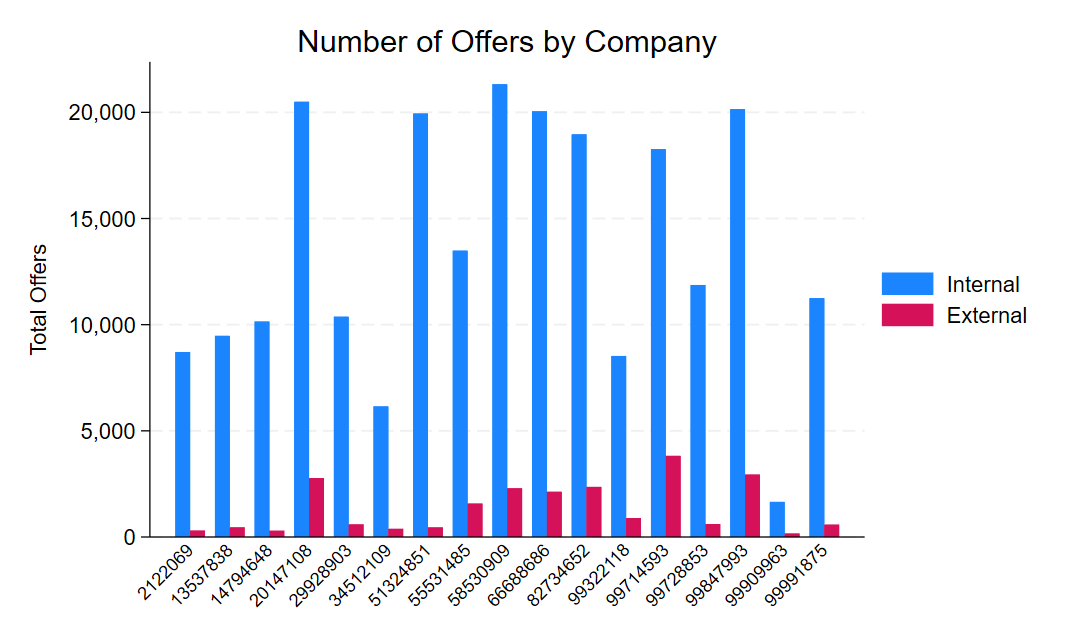
\includegraphics[scale=0.27]{figures/IE4/IE4_int_ext_offers_by_cia.png} 
\end{tabular}
\end{figure}

\begin{figure}[H]
\caption{}
 \label{fig:ie4_2and3}
\centering{}%
\begin{tabular}{cc}
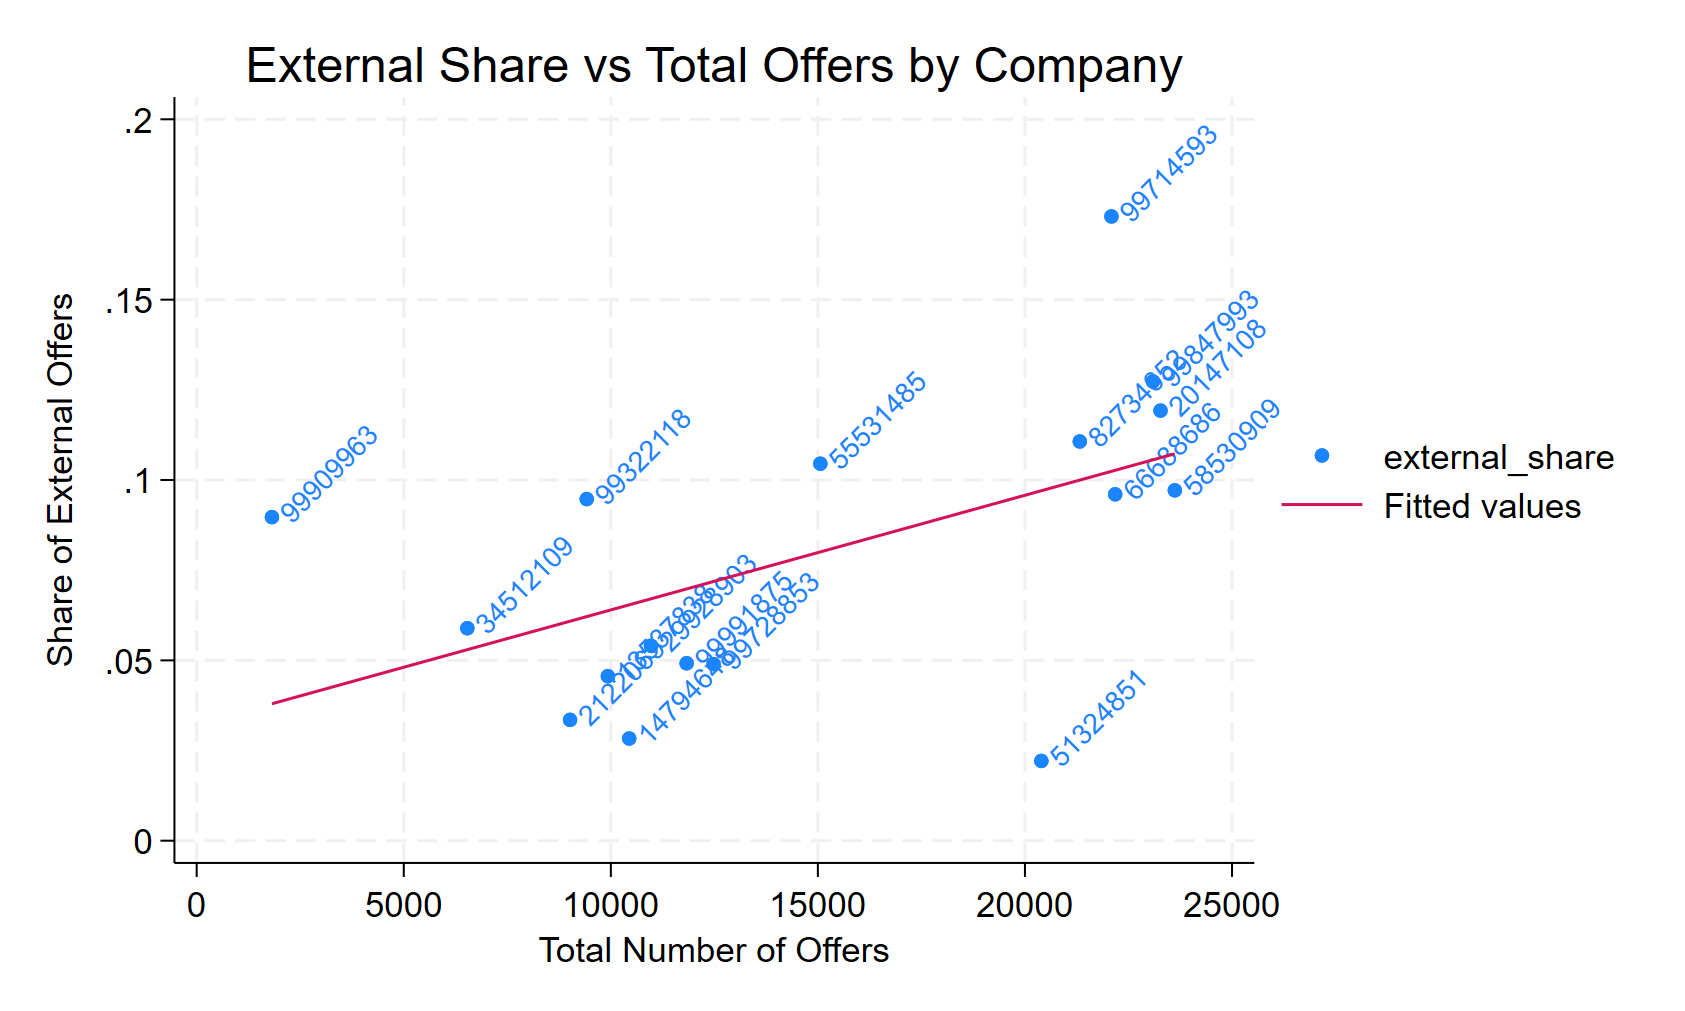
\includegraphics[scale=0.27]{figures/IE4/IE4_total_internal_offers_bycompany.png} & 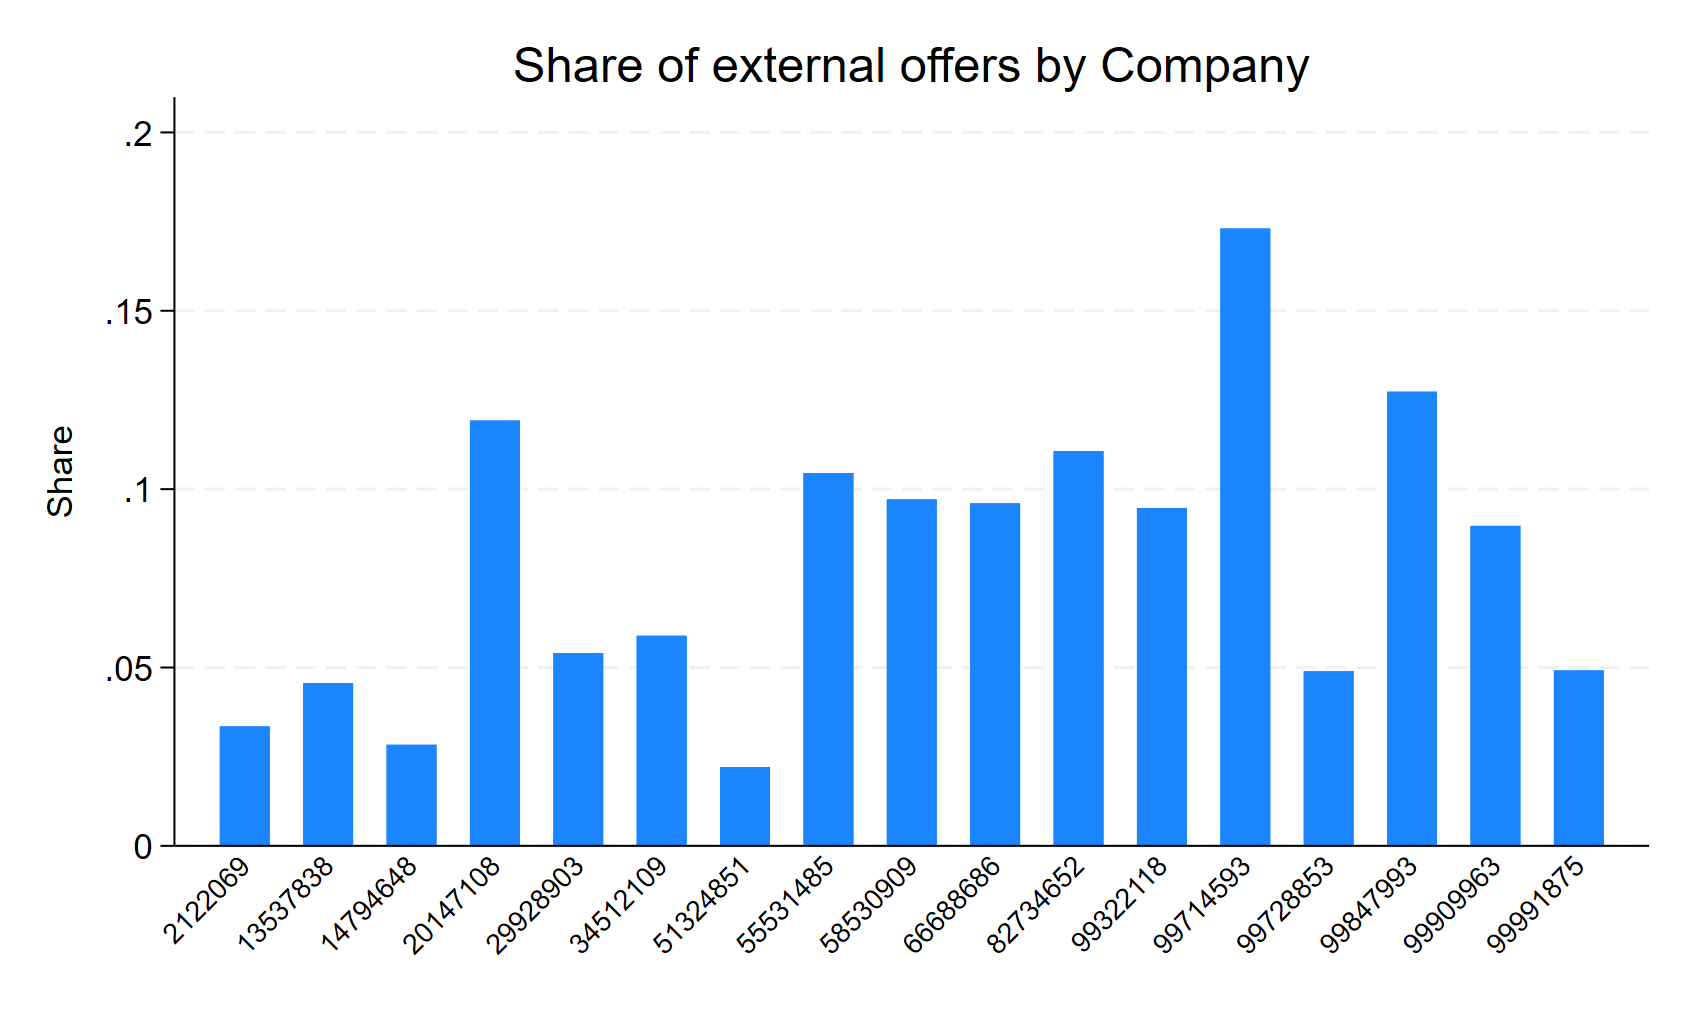
\includegraphics[scale=0.27]{figures/IE4/IE4_variation_share_external.png}
\end{tabular}
\end{figure} 

\newpage

\subsection{Negative correlation credit rating and offers}

Offers with better credit ratings make worse offers, this could reflect cost issues or a less elastic demand. 

\begin{figure}[H]
\caption{}
 \label{fig:ie4_4}
\centering{}%
\begin{tabular}{cc}
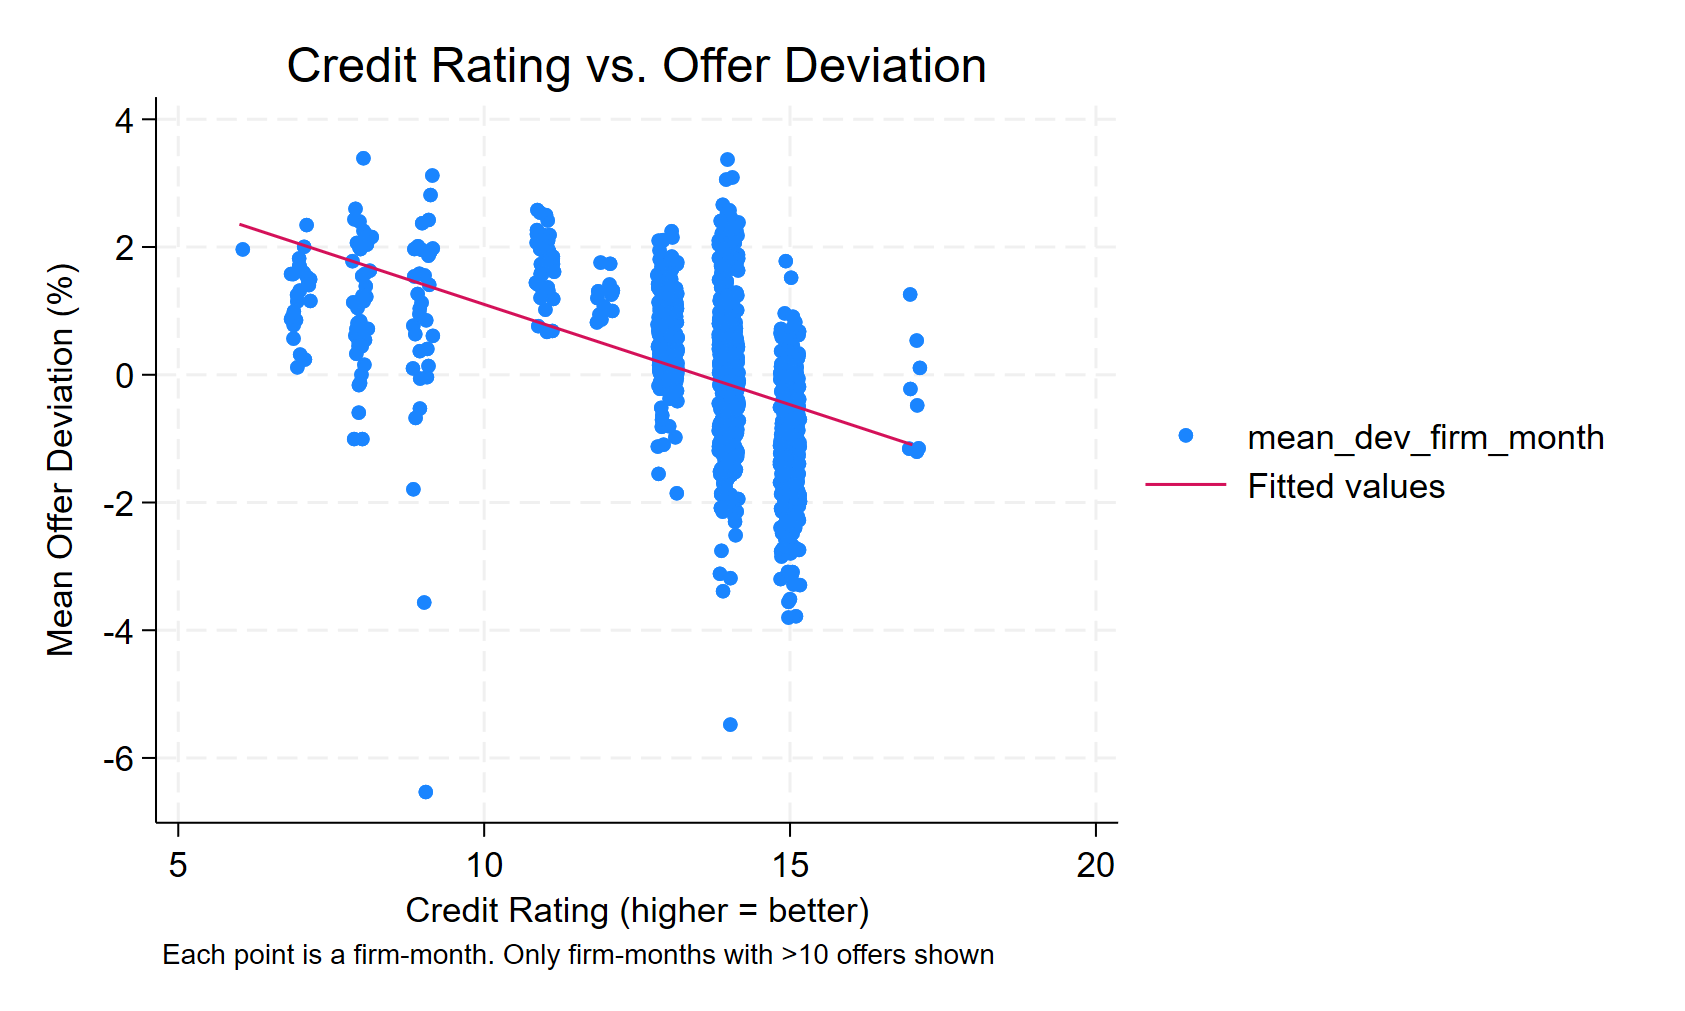
\includegraphics[scale=0.27]{figures/IE4/IE4_scatter_rating_offer.png} 
\end{tabular}
\end{figure}

\begin{figure}[H]
\caption{}
 \label{fig:ie4_5and6}
\centering{}%
\begin{tabular}{cc}
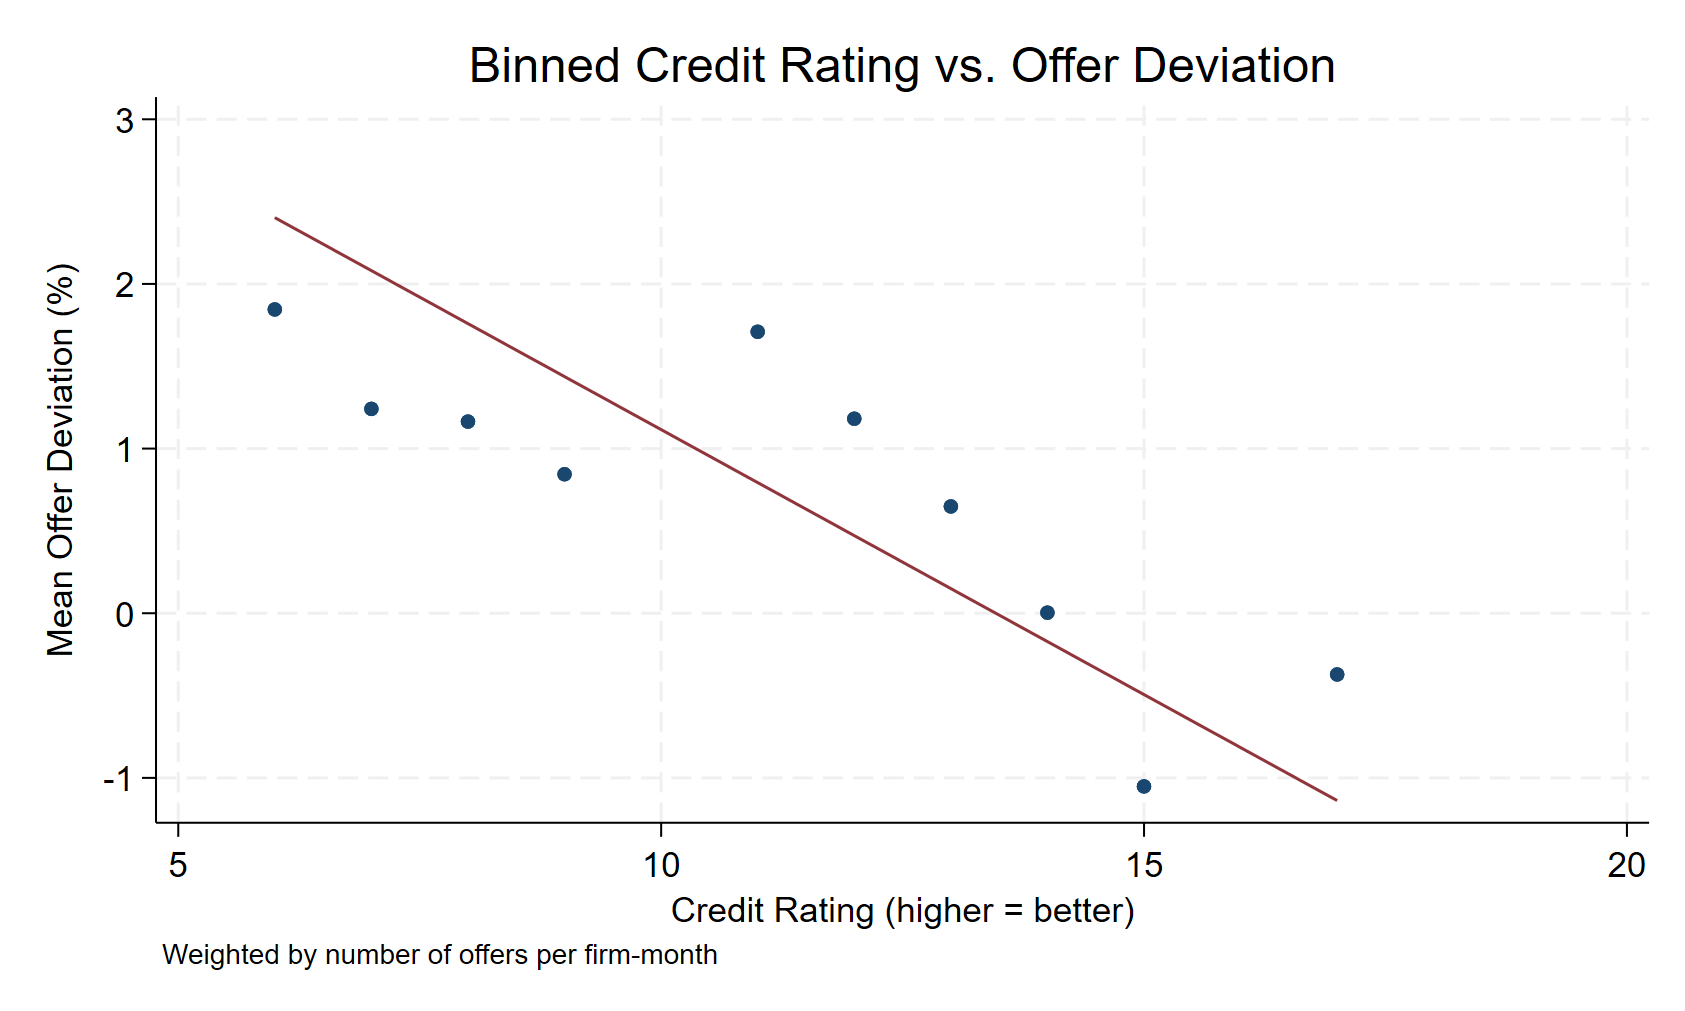
\includegraphics[scale=0.27]{figures/IE4/IE4_binscatter_rating_offer.png} & 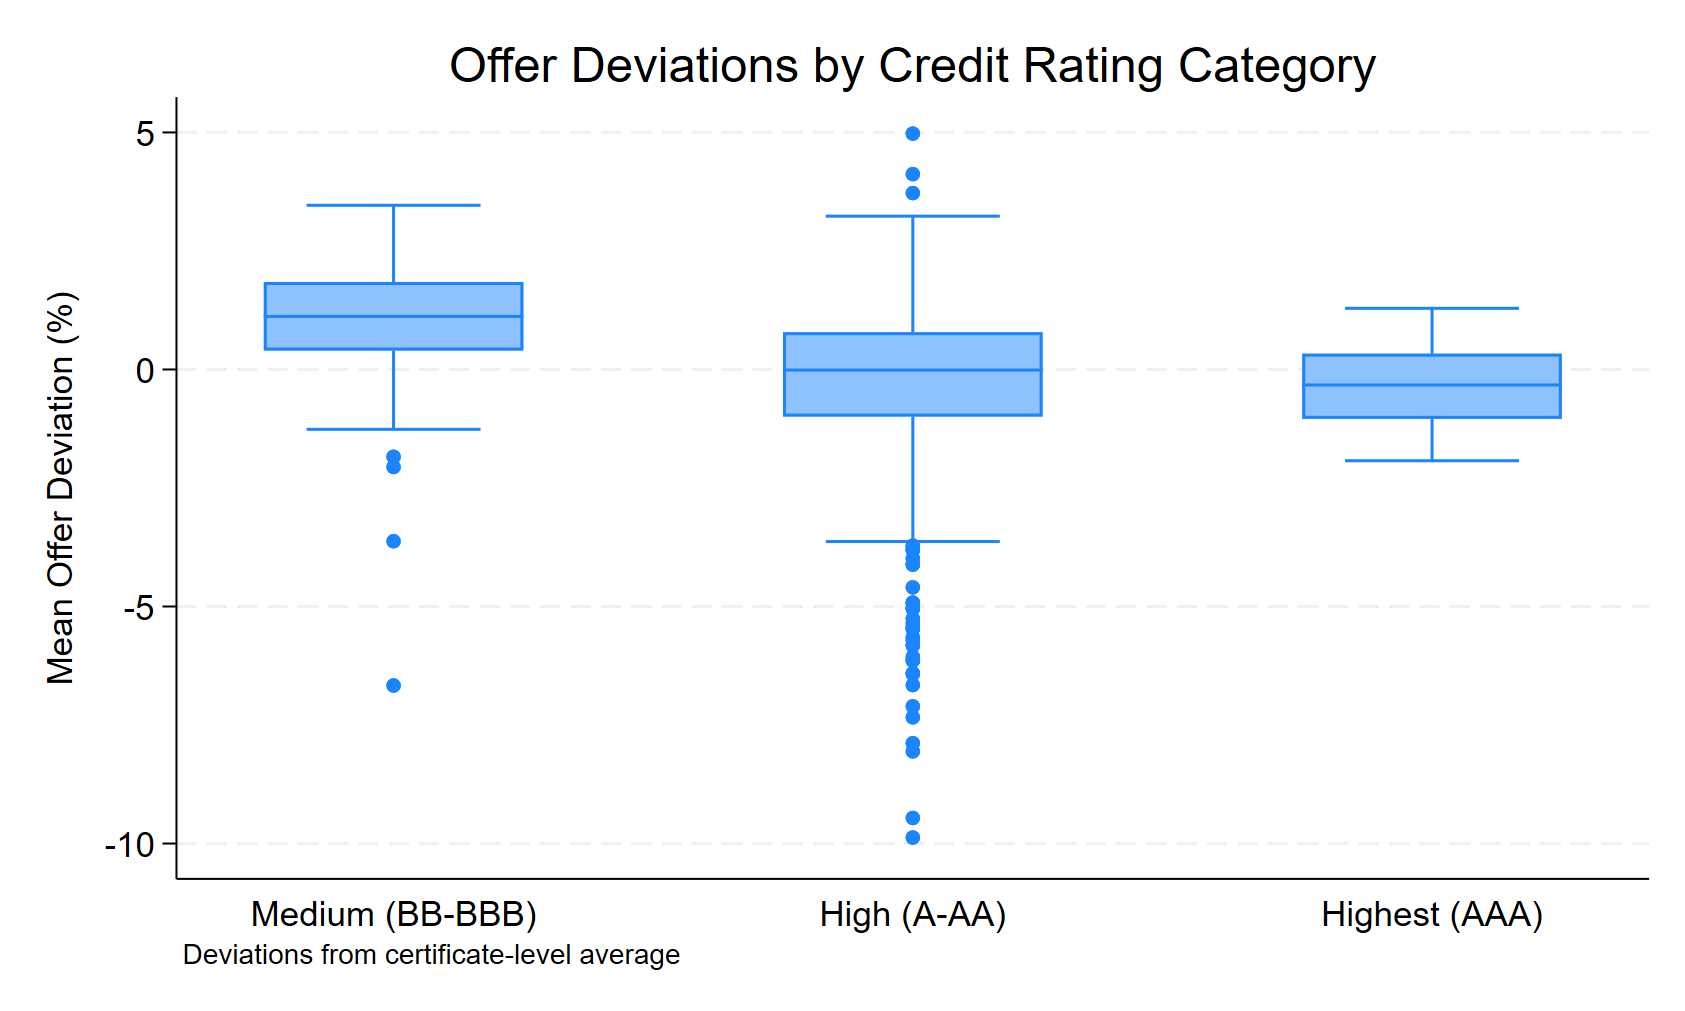
\includegraphics[scale=0.27]{figures/IE4/IE4_box_rating_offer.png}
\end{tabular}
\end{figure}



Correlation: 
Coefficient: -0.322 (SE:  0.017)



\newpage

\subsection{Intermediaries and external offers}



\begin{figure}[H]
\caption{}
 \label{fig:ie4_6and7}
\centering{}%
\begin{tabular}{cc}
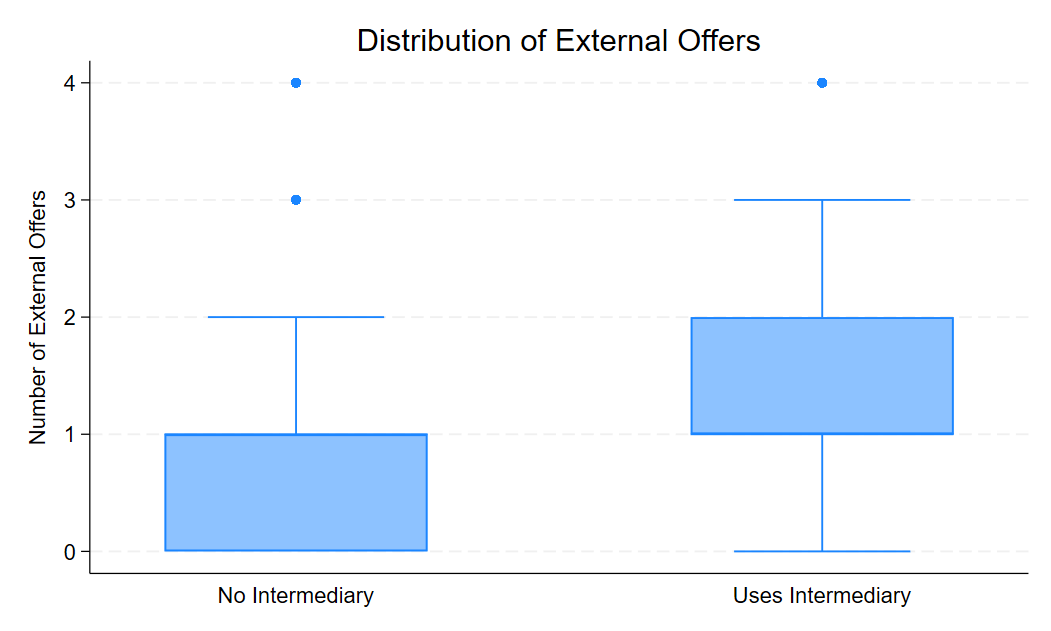
\includegraphics[scale=0.27]{figures/IE4/IE4_intermediary_search_box.png} 
\end{tabular}
\end{figure}

\begin{table}[htbp]\centering
\def\sym#1{\ifmmode^{#1}\else\(^{#1}\)\fi}
\caption{Search Intensity by Intermediary Use}
\begin{tabular}{l*{1}{ccccc}}
\hline\hline
            &No Intermediary&Has Intermediary&  Difference         & t-statistic&     p-value\\
\hline
n\_ext       &     1.08645&    1.566799&   -.4803491\sym{***}&   -25.95889&    2.3e-146\\
\hline
\(N\)       &       21956&            &                     &            &            \\
\hline\hline
\end{tabular}
\end{table}



\newpage

\subsection{Intermediaries and external offers(2)}

\begin{table}[htbp]\centering
\def\sym#1{\ifmmode^{#1}\else\(^{#1}\)\fi}
\caption{Search Behavior by Intermediary Status}
\begin{tabular}{l*{1}{cccc}}
\hline\hline
            &        mean&          sd&         min&       count\\
\hline
0           &            &            &            &            \\
n\_external  &        1.09&        1.33&           0&       10908\\
n\_internal  &       14.09&        7.26&           0&       10908\\
n\_total\_offers&       15.17&        7.75&           1&       10908\\
chose\_external&        0.61&        0.49&           0&       10908\\
\hline
1           &            &            &            &            \\
n\_external  &        1.57&        1.41&           0&       11048\\
n\_internal  &       14.96&        8.81&           0&       11048\\
n\_total\_offers&       16.52&        9.33&           1&       11048\\
chose\_external&        0.91&        0.29&           0&       11048\\
\hline
Total       &            &            &            &            \\
n\_external  &        1.33&        1.39&           0&       21956\\
n\_internal  &       14.52&        8.09&           0&       21956\\
n\_total\_offers&       15.85&        8.61&           1&       21956\\
chose\_external&        0.76&        0.43&           0&       21956\\
\hline
\(N\)       &       21956&            &            &            \\
\hline\hline
\multicolumn{5}{l}{\footnotesize number of searches}\\
\end{tabular}
\end{table}


\begin{table}[htbp]\centering
\def\sym#1{\ifmmode^{#1}\else\(^{#1}\)\fi}
\caption{External Offers by Intermediary Type}
\begin{tabular}{l*{2}{ccc}}
\hline\hline
            &        mean&          sd&       count&        mean&          sd&       count\\
\hline
\hline
\(N\)       &       21956&            &            &       21956&            &            \\
\hline\hline
\end{tabular}
\end{table}


 

 

 
\begin{figure}[H]
\caption{}
 \label{fig:ie4_7and8}
\centering{}%
\begin{tabular}{cc}
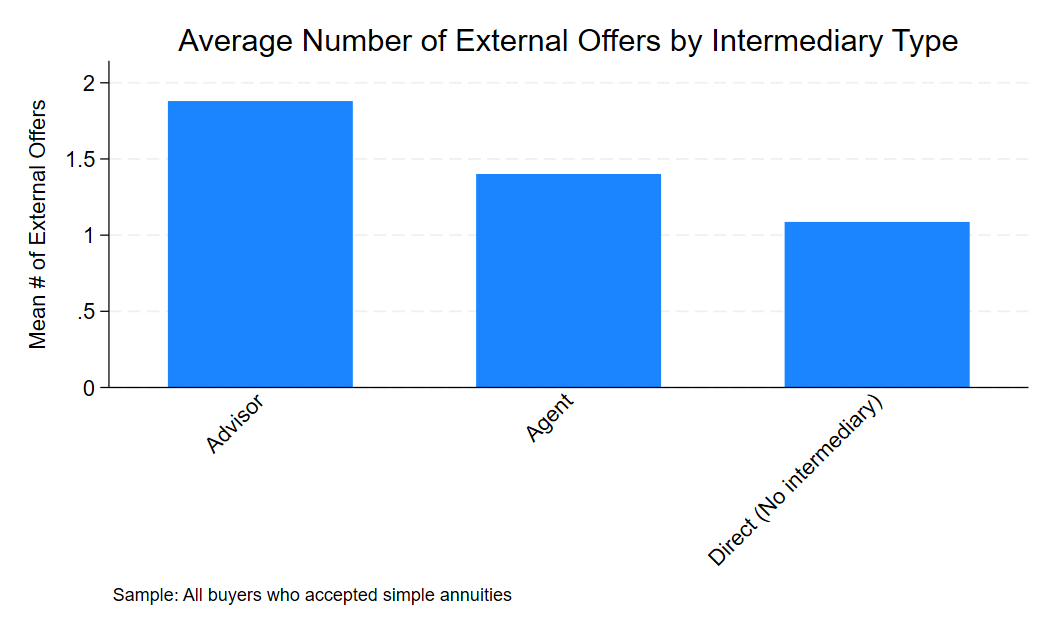
\includegraphics[scale=0.27]{figures/IE4/IE4_external_offers_by_intermediary.png} & 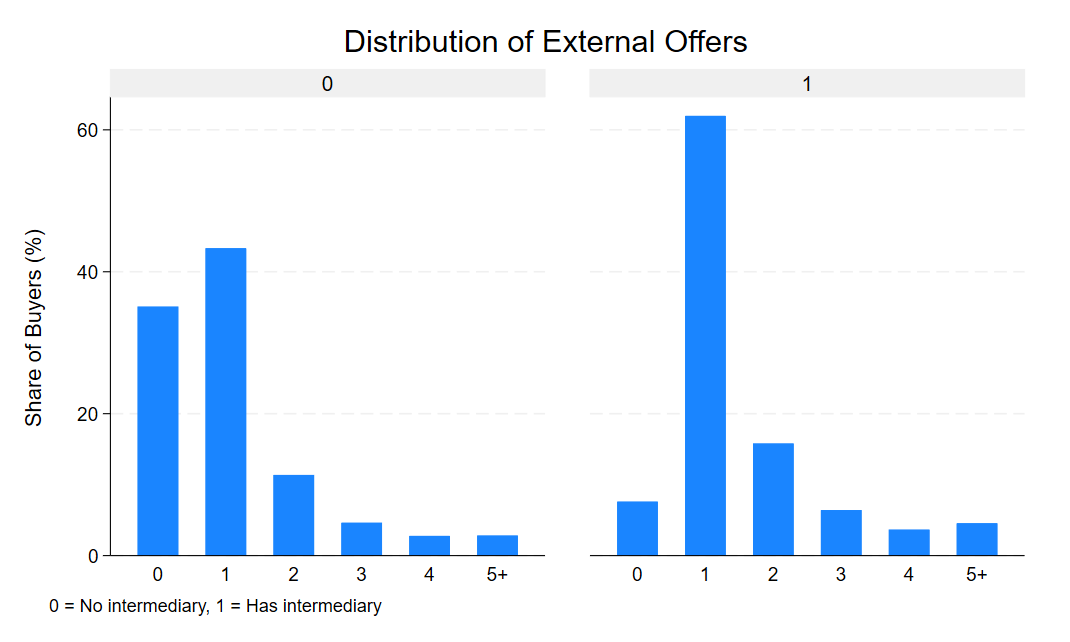
\includegraphics[scale=0.27]{figures/IE4/IE4_external_distribution_by_intermediary.png} 
\end{tabular}
\end{figure} 
 
\begin{figure}[H]
\caption{}
 \label{fig:ie4_9and10}
\centering{}%
\begin{tabular}{cc}
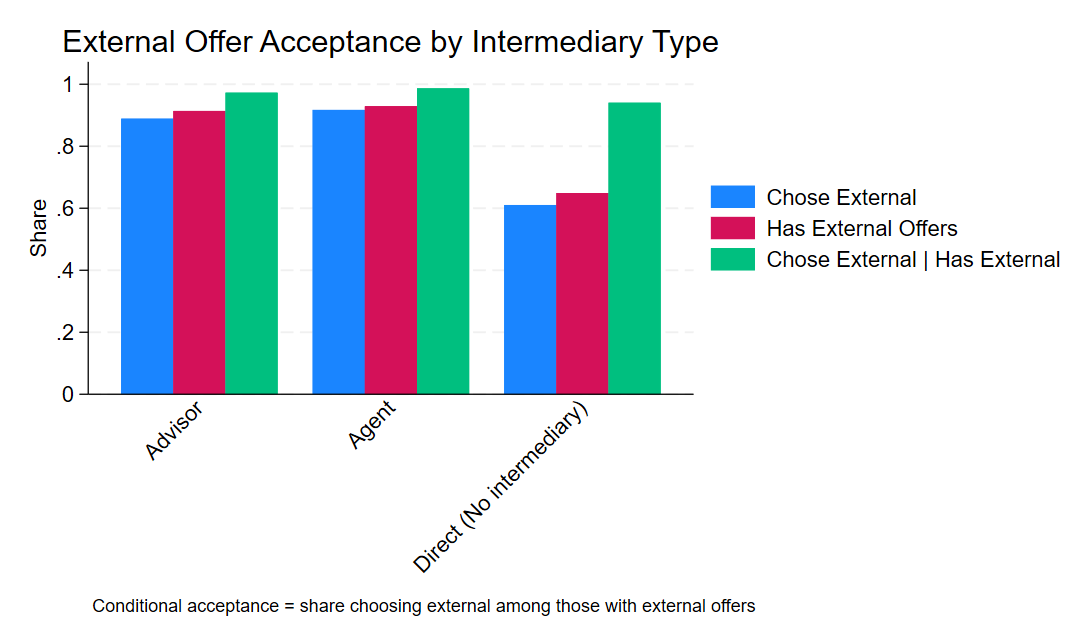
\includegraphics[scale=0.27]{figures/IE4/IE4_external_acceptance_by_intermediary.png} 
\end{tabular}
\end{figure} 
 
 \input{Tables/ie4/ie4_regression_external.tex}
  \begin{table}[htbp]\centering
\def\sym#1{\ifmmode^{#1}\else\(^{#1}\)\fi}
\caption{Probability of Choosing External Offer (Conditional on Having External)}
\begin{tabular}{l*{2}{c}}
\hline\hline
                    &\multicolumn{1}{c}{(1)}         &\multicolumn{1}{c}{(2)}         \\
\hline
chose\_external      &                     &                     \\
has\_intermediary    &       1.245\sym{***}&                     \\
                    &     (0.090)         &                     \\
[1em]
A                   &                     &       0.000         \\
                    &                     &         (.)         \\
[1em]
D                   &                     &      -1.562\sym{***}\\
                    &                     &     (0.118)         \\
[1em]
P                   &                     &      -0.742\sym{***}\\
                    &                     &     (0.149)         \\
[1em]
Constant            &       2.759\sym{***}&       4.321\sym{***}\\
                    &     (0.050)         &     (0.107)         \\
\hline
Obs.                &      17,289         &      17,289         \\
\hline\hline
\end{tabular}
\end{table}


  \begin{figure}[H]
\caption{}
 \label{fig:ie4_11}
\centering{}%
\begin{tabular}{cc}
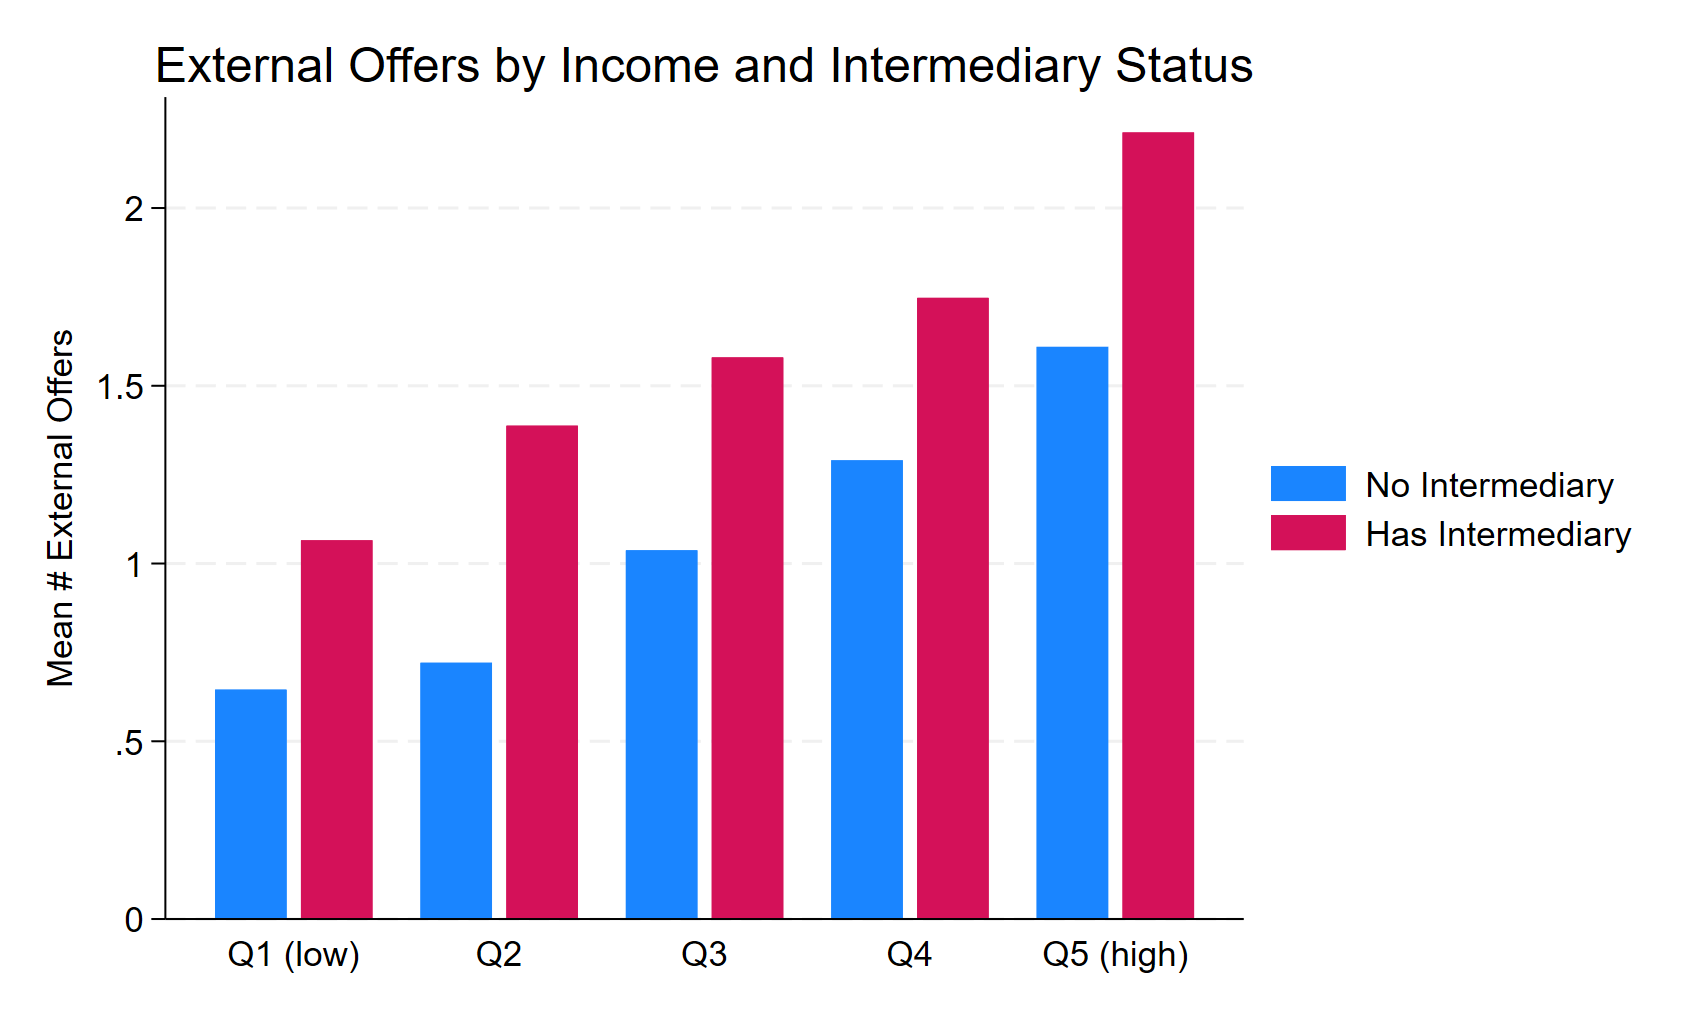
\includegraphics[scale=0.27]{figures/IE4/IE4_external_by_income_intermediary.png} 
\end{tabular}
\end{figure} 

\newpage

\subsection{Choose highest offer and Intermediaries}
 Share choosing highest offer:  0.544
Mean foregone value (% of chosen):   1.62


\begin{table}[htbp]\centering
\def\sym#1{\ifmmode^{#1}\else\(^{#1}\)\fi}
\caption{Choosing Highest Offer by Income Quintile}
\begin{tabular}{l*{1}{ccc}}
\hline\hline
            &        mean&          sd&       count\\
\hline
Q1(low)     &            &            &            \\
chose\_highest\_cert&       0.516&       0.500&        3700\\
foregone\_pct&       1.076&       1.585&        3700\\
foregone\_pct2&       2.222&       1.626&        1791\\
n\_total\_offers&       7.571&       4.231&        3700\\
\hline
Q2          &            &            &            \\
chose\_highest\_cert&       0.550&       0.498&        3659\\
foregone\_pct&       0.674&       1.094&        3659\\
foregone\_pct2&       1.497&       1.195&        1648\\
n\_total\_offers&      12.286&       4.705&        3659\\
\hline
Q3          &            &            &            \\
chose\_highest\_cert&       0.574&       0.495&        3644\\
foregone\_pct&       0.568&       0.999&        3644\\
foregone\_pct2&       1.332&       1.151&        1554\\
n\_total\_offers&      15.037&       5.649&        3644\\
\hline
Q4          &            &            &            \\
chose\_highest\_cert&       0.576&       0.494&        3640\\
foregone\_pct&       0.594&       1.121&        3640\\
foregone\_pct2&       1.402&       1.355&        1542\\
n\_total\_offers&      17.129&       6.833&        3640\\
\hline
Q5(high)    &            &            &            \\
chose\_highest\_cert&       0.505&       0.500&        3649\\
foregone\_pct&       0.782&       1.348&        3649\\
foregone\_pct2&       1.579&       1.553&        1807\\
n\_total\_offers&      17.362&       7.377&        3649\\
\hline
Total       &            &            &            \\
chose\_highest\_cert&       0.544&       0.498&       18292\\
foregone\_pct&       0.740&       1.262&       18292\\
foregone\_pct2&       1.622&       1.436&        8342\\
n\_total\_offers&      13.857&       6.920&       18292\\
\hline
\(N\)       &       18292&            &            \\
\hline\hline
\end{tabular}
\end{table}


  \begin{figure}[H]
\caption{}
 \label{fig:ie4_12}
\centering{}%
\begin{tabular}{cc}
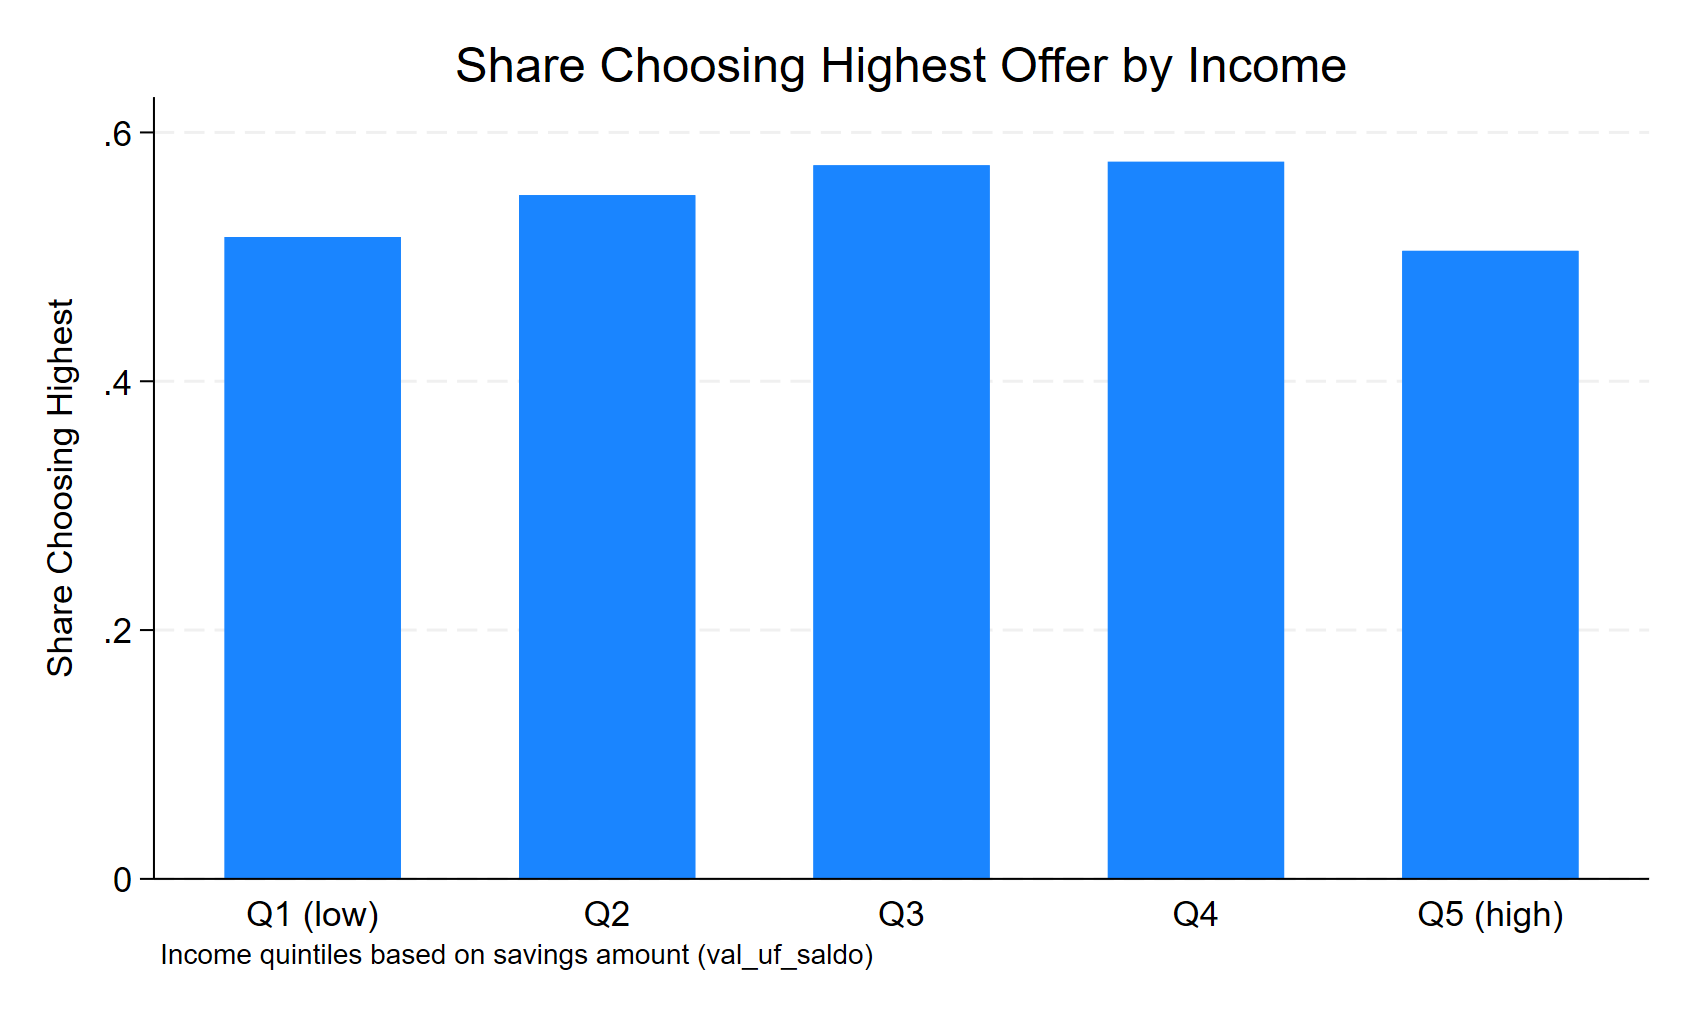
\includegraphics[scale=0.27]{figures/IE4/IE4_highest_by_income.png} 
\end{tabular}
\end{figure} 

 \begin{table}[htbp]\centering
\def\sym#1{\ifmmode^{#1}\else\(^{#1}\)\fi}
\caption{Choosing Highest Offer by Intermediary Status}
\begin{tabular}{l*{1}{ccc}}
\hline\hline
            &        mean&          sd&       count\\
\hline
0           &            &            &            \\
chose\_highest\_cert&       0.629&       0.483&        9507\\
foregone\_pct&       0.518&       1.047&        9507\\
foregone\_pct2&       1.398&       1.315&        3524\\
n\_total\_offers&      13.501&       6.185&        9507\\
\hline
1           &            &            &            \\
chose\_highest\_cert&       0.452&       0.498&        8785\\
foregone\_pct&       0.979&       1.421&        8785\\
foregone\_pct2&       1.786&       1.498&        4818\\
n\_total\_offers&      14.242&       7.618&        8785\\
\hline
Total       &            &            &            \\
chose\_highest\_cert&       0.544&       0.498&       18292\\
foregone\_pct&       0.740&       1.262&       18292\\
foregone\_pct2&       1.622&       1.436&        8342\\
n\_total\_offers&      13.857&       6.920&       18292\\
\hline
\(N\)       &       18292&            &            \\
\hline\hline
\end{tabular}
\end{table}




   \begin{figure}[H]
\caption{}
 \label{fig:ie4_11}
\centering{}%
\begin{tabular}{cc}
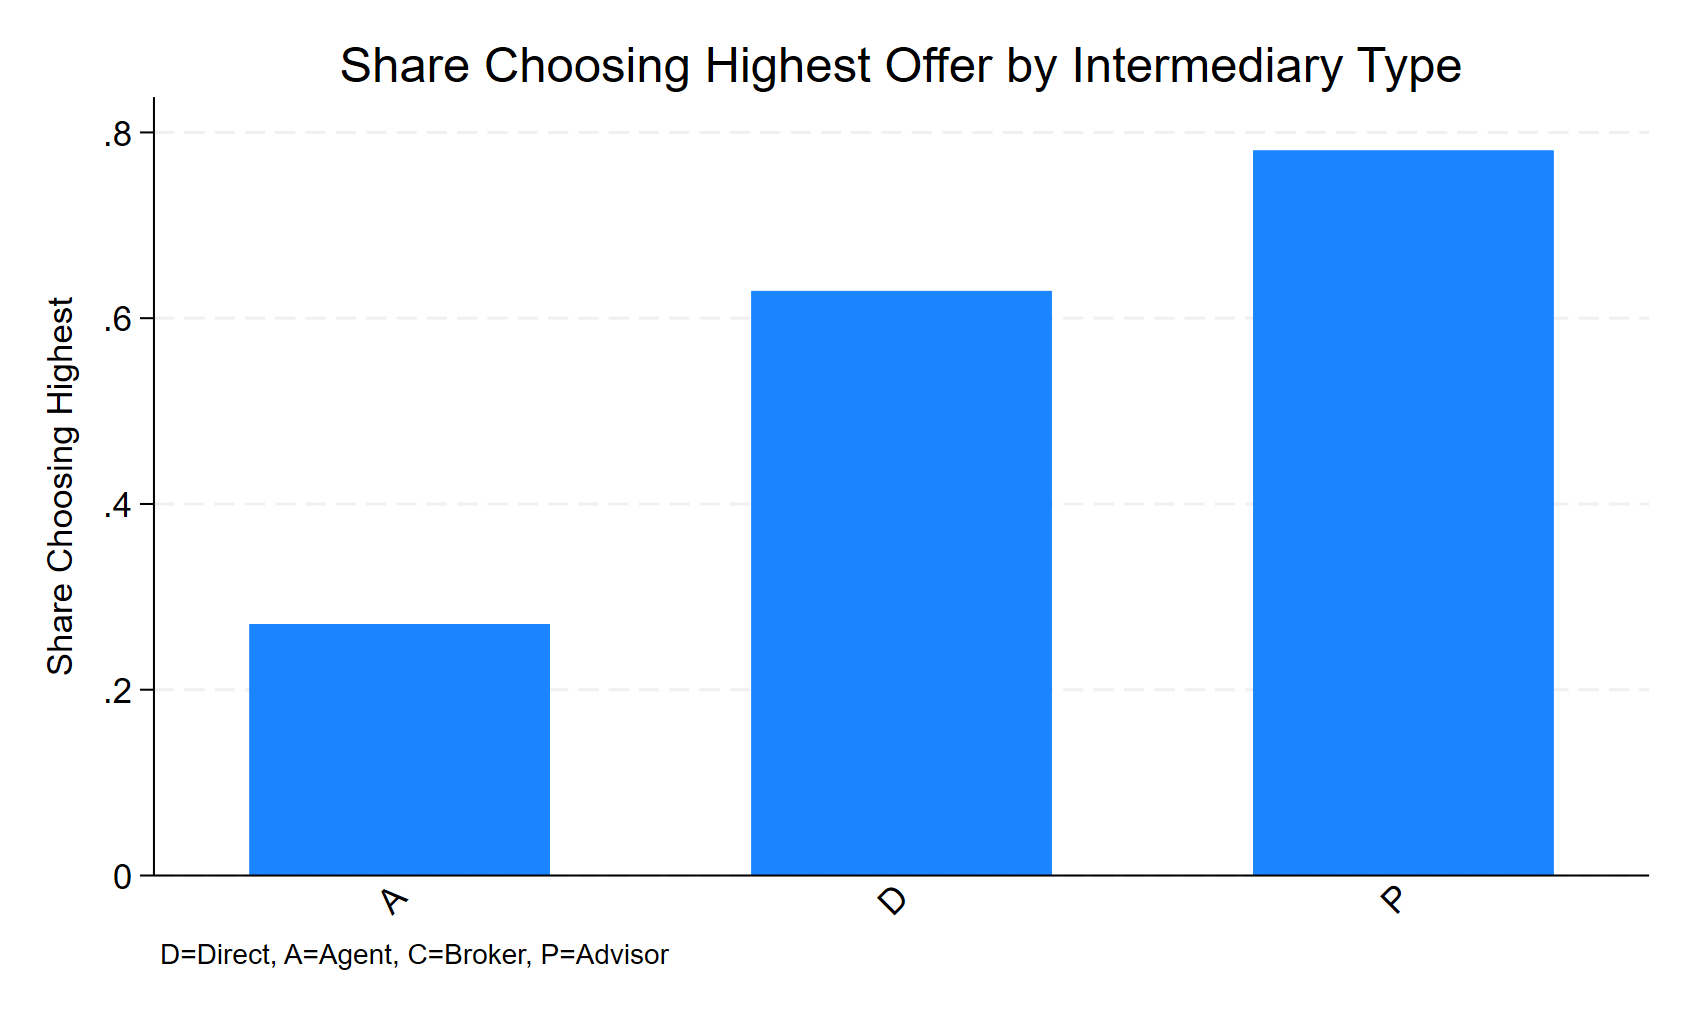
\includegraphics[scale=0.27]{figures/IE4/IE4_highest_by_intermediary_type.png} 
& 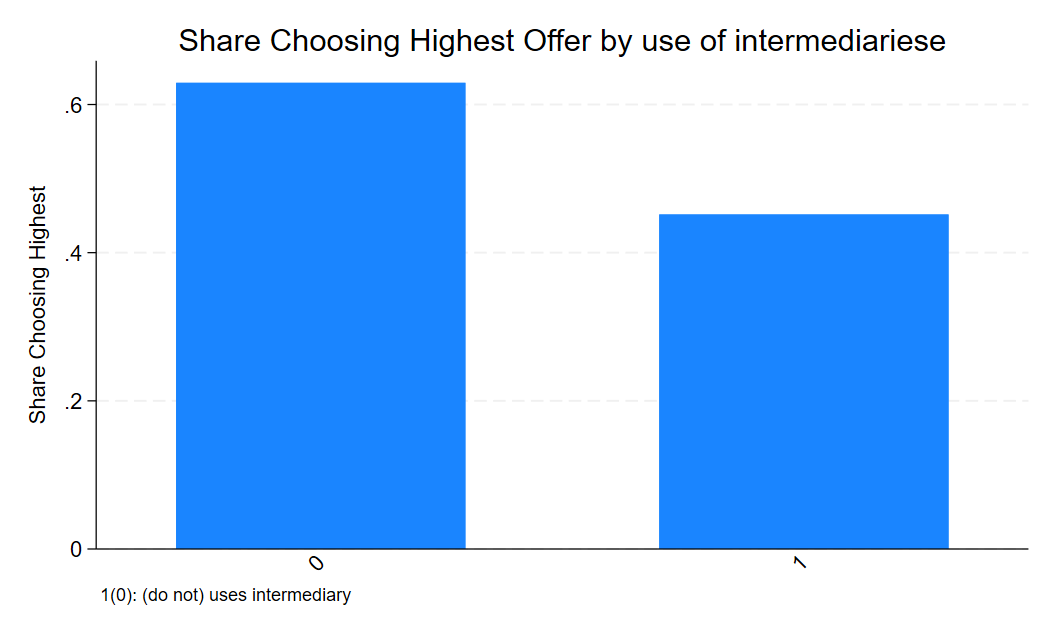
\includegraphics[scale=0.27]{figures/IE4/IE4_highest_by_intermediary_type(2).png} 
\end{tabular}
\end{figure} 
 

\begin{table}[htbp]\centering
\def\sym#1{\ifmmode^{#1}\else\(^{#1}\)\fi}
\caption{Choosing Highest Offer by External Offer Status}
\begin{tabular}{l*{6}{ccc}}
\hline\hline
            &        mean&          sd&       count&        mean&          sd&       count&        mean&          sd&       count&        mean&          sd&       count&        mean&          sd&       count&        mean&          sd&       count\\
\hline
\hline
\(N\)       &       18292&            &            &       18292&            &            &       18292&            &            &       18292&            &            &       18292&            &            &        8342&            &            \\
\hline\hline
\end{tabular}
\end{table}



  \begin{figure}[H]
\caption{}
 \label{fig:ie4_11}
\centering{}%
\begin{tabular}{cc}
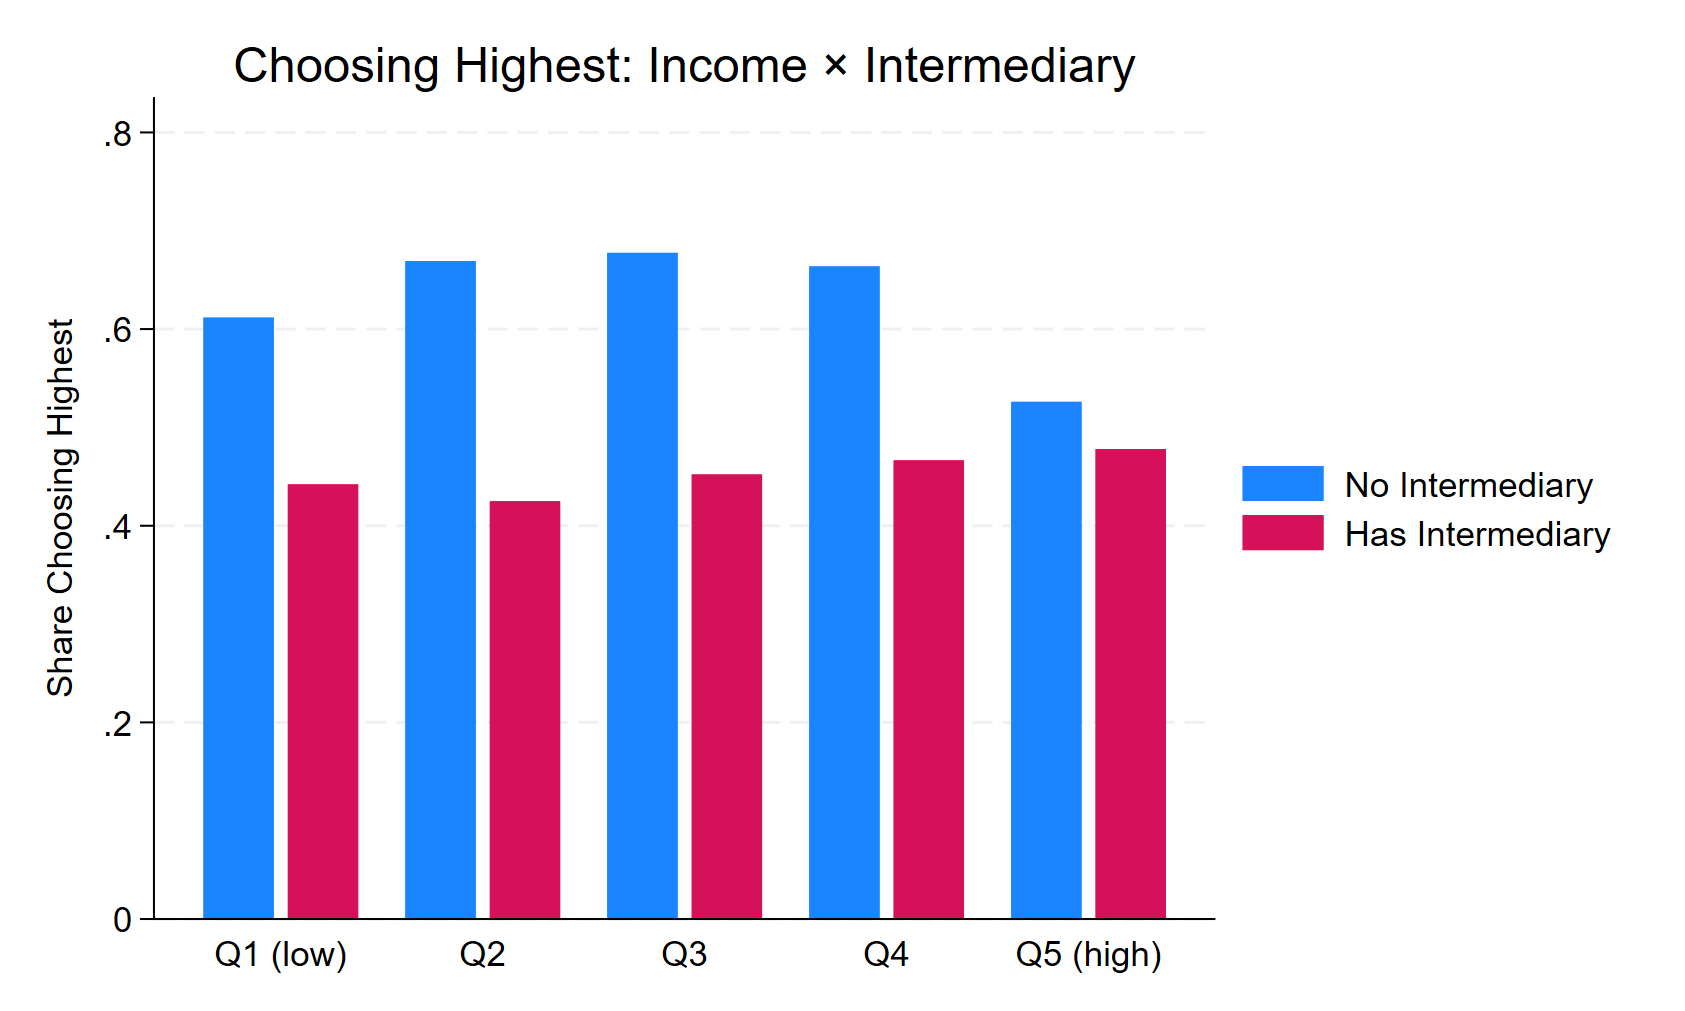
\includegraphics[scale=0.27]{figures/IE4/IE4_highest_income_intermediary.png} & 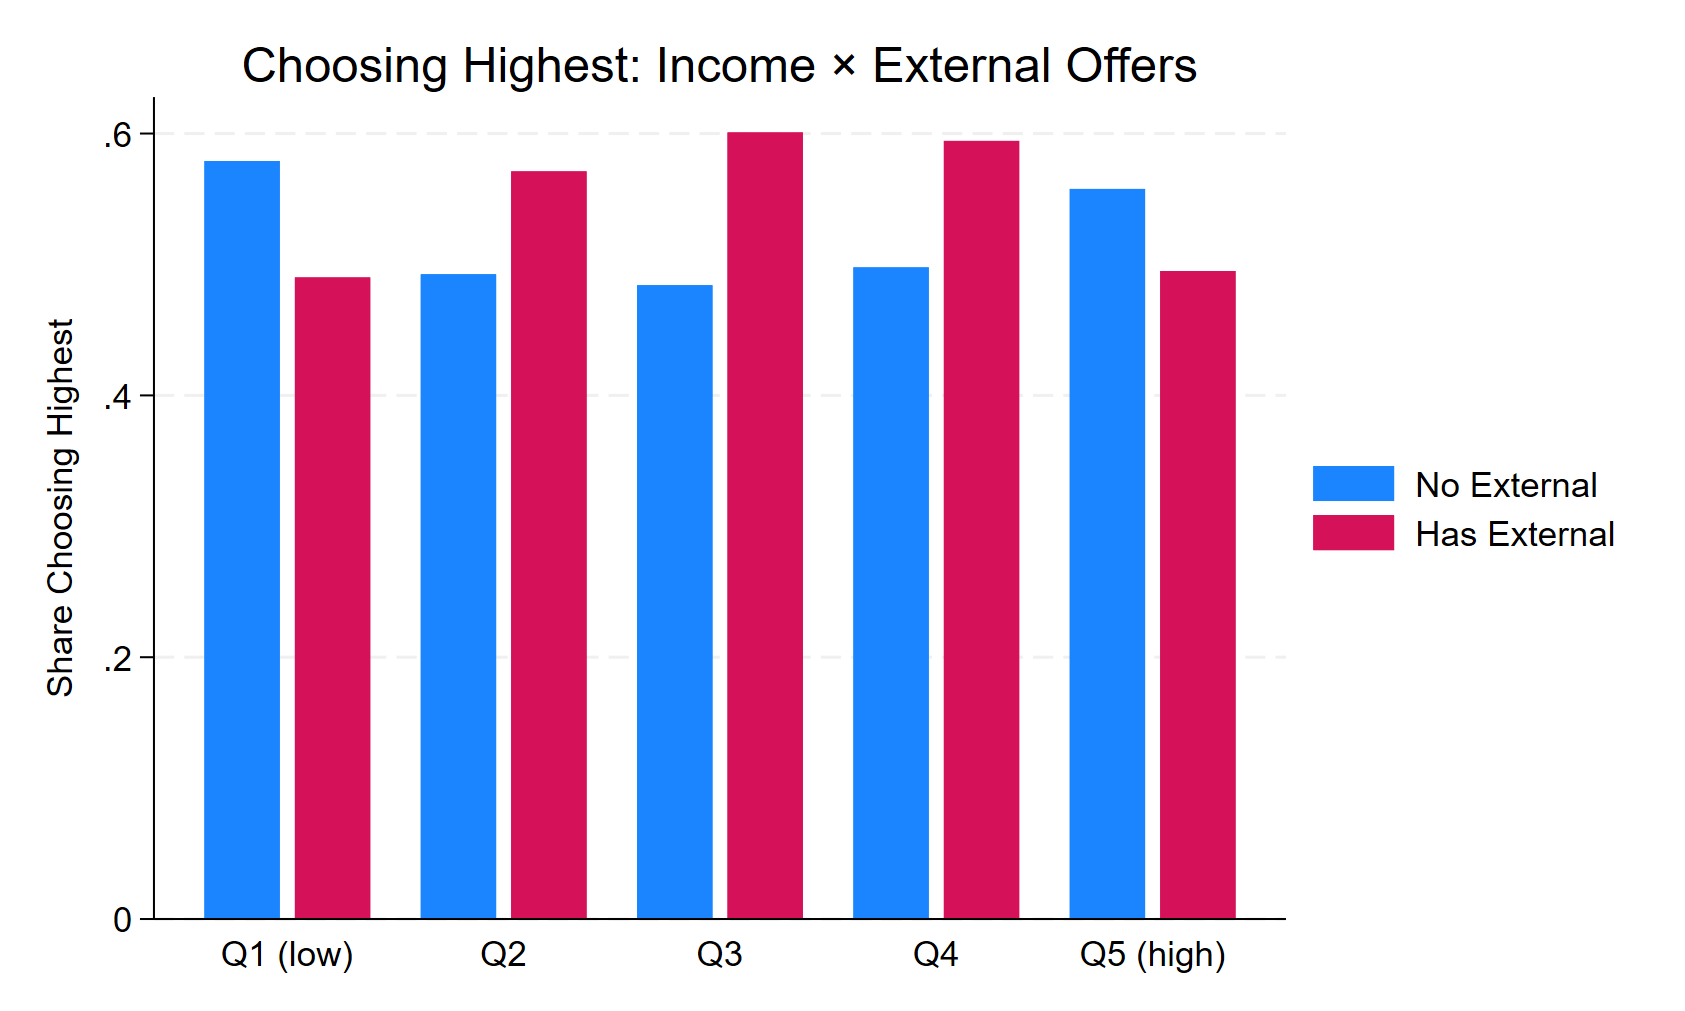
\includegraphics[scale=0.27]{figures/IE4/IE4_highest_income_external.png} 
\end{tabular}
\end{figure} 


%\begin{table}[htbp]\centering
\def\sym#1{\ifmmode^{#1}\else\(^{#1}\)\fi}
\caption{Determinants of Choosing Highest Offer}
\begin{tabular}{l*{5}{c}}
\hline\hline
            &\multicolumn{1}{c}{(1)}         &\multicolumn{1}{c}{(2)}         &\multicolumn{1}{c}{(3)}         &\multicolumn{1}{c}{(4)}         &\multicolumn{1}{c}{(5)}         \\
\hline
main        &                     &                     &                     &                     &                     \\
has\_intermediary&      -0.867\sym{***}&      -0.879\sym{***}&      -0.873\sym{***}&                     &      -0.209\sym{***}\\
            &     (0.033)         &     (0.033)         &     (0.033)         &                     &     (0.008)         \\
[1em]
has\_external&       0.475\sym{***}&       0.498\sym{***}&       0.418\sym{***}&                     &       0.098\sym{***}\\
            &     (0.040)         &     (0.040)         &     (0.046)         &                     &     (0.011)         \\
[1em]
1.income\_q  &                     &       0.000         &       0.000         &       0.000         &       0.000         \\
            &                     &         (.)         &         (.)         &         (.)         &         (.)         \\
[1em]
2.income\_q  &                     &       0.066         &       0.207\sym{***}&       0.211\sym{***}&       0.049\sym{***}\\
            &                     &     (0.048)         &     (0.049)         &     (0.049)         &     (0.012)         \\
[1em]
3.income\_q  &                     &       0.122\sym{**} &       0.337\sym{***}&       0.335\sym{***}&       0.079\sym{***}\\
            &                     &     (0.048)         &     (0.052)         &     (0.052)         &     (0.012)         \\
[1em]
4.income\_q  &                     &       0.095\sym{*}  &       0.360\sym{***}&       0.351\sym{***}&       0.085\sym{***}\\
            &                     &     (0.048)         &     (0.055)         &     (0.055)         &     (0.013)         \\
[1em]
5.income\_q  &                     &      -0.222\sym{***}&       0.009         &       0.026         &       0.003         \\
            &                     &     (0.049)         &     (0.056)         &     (0.056)         &     (0.013)         \\
[1em]
n\_total\_offers&                     &                     &      -0.033\sym{***}&      -0.025\sym{***}&      -0.008\sym{***}\\
            &                     &                     &     (0.003)         &     (0.003)         &     (0.001)         \\
[1em]
n\_external  &                     &                     &       0.112\sym{***}&                     &       0.026\sym{***}\\
            &                     &                     &     (0.017)         &                     &     (0.004)         \\
[1em]
0.has\_intermediary&                     &                     &                     &       0.000         &                     \\
            &                     &                     &                     &         (.)         &                     \\
[1em]
1.has\_intermediary&                     &                     &                     &       0.028         &                     \\
            &                     &                     &                     &     (0.083)         &                     \\
[1em]
0.has\_external&                     &                     &                     &       0.000         &                     \\
            &                     &                     &                     &         (.)         &                     \\
[1em]
1.has\_external&                     &                     &                     &       0.809\sym{***}&                     \\
            &                     &                     &                     &     (0.045)         &                     \\
[1em]
0.has\_intermediary#0.has\_external&                     &                     &                     &       0.000         &                     \\
            &                     &                     &                     &         (.)         &                     \\
[1em]
0.has\_intermediary#1.has\_external&                     &                     &                     &       0.000         &                     \\
            &                     &                     &                     &         (.)         &                     \\
[1em]
1.has\_intermediary#0.has\_external&                     &                     &                     &       0.000         &                     \\
            &                     &                     &                     &         (.)         &                     \\
[1em]
1.has\_intermediary#1.has\_external&                     &                     &                     &      -1.056\sym{***}&                     \\
            &                     &                     &                     &     (0.090)         &                     \\
[1em]
\_cons      &       0.235\sym{***}&       0.211\sym{***}&       0.416\sym{***}&       0.181\sym{***}&       0.600\sym{***}\\
            &     (0.032)         &     (0.044)         &     (0.047)         &     (0.048)         &     (0.011)         \\
\hline
Obs.        &      18,292         &      18,292         &      18,292         &      18,292         &      18,292         \\
Pseudo R2   &       0.029         &       0.032         &       0.038         &       0.041         &                     \\
\hline\hline
\multicolumn{6}{l}{\footnotesize Models 1-4: Logit. Model 5: LPM. Robust standard errors.}\\
\end{tabular}
\end{table}





  \begin{figure}[H]
\caption{}
 \label{fig:ie4_11}
\centering{}%
\begin{tabular}{cc}
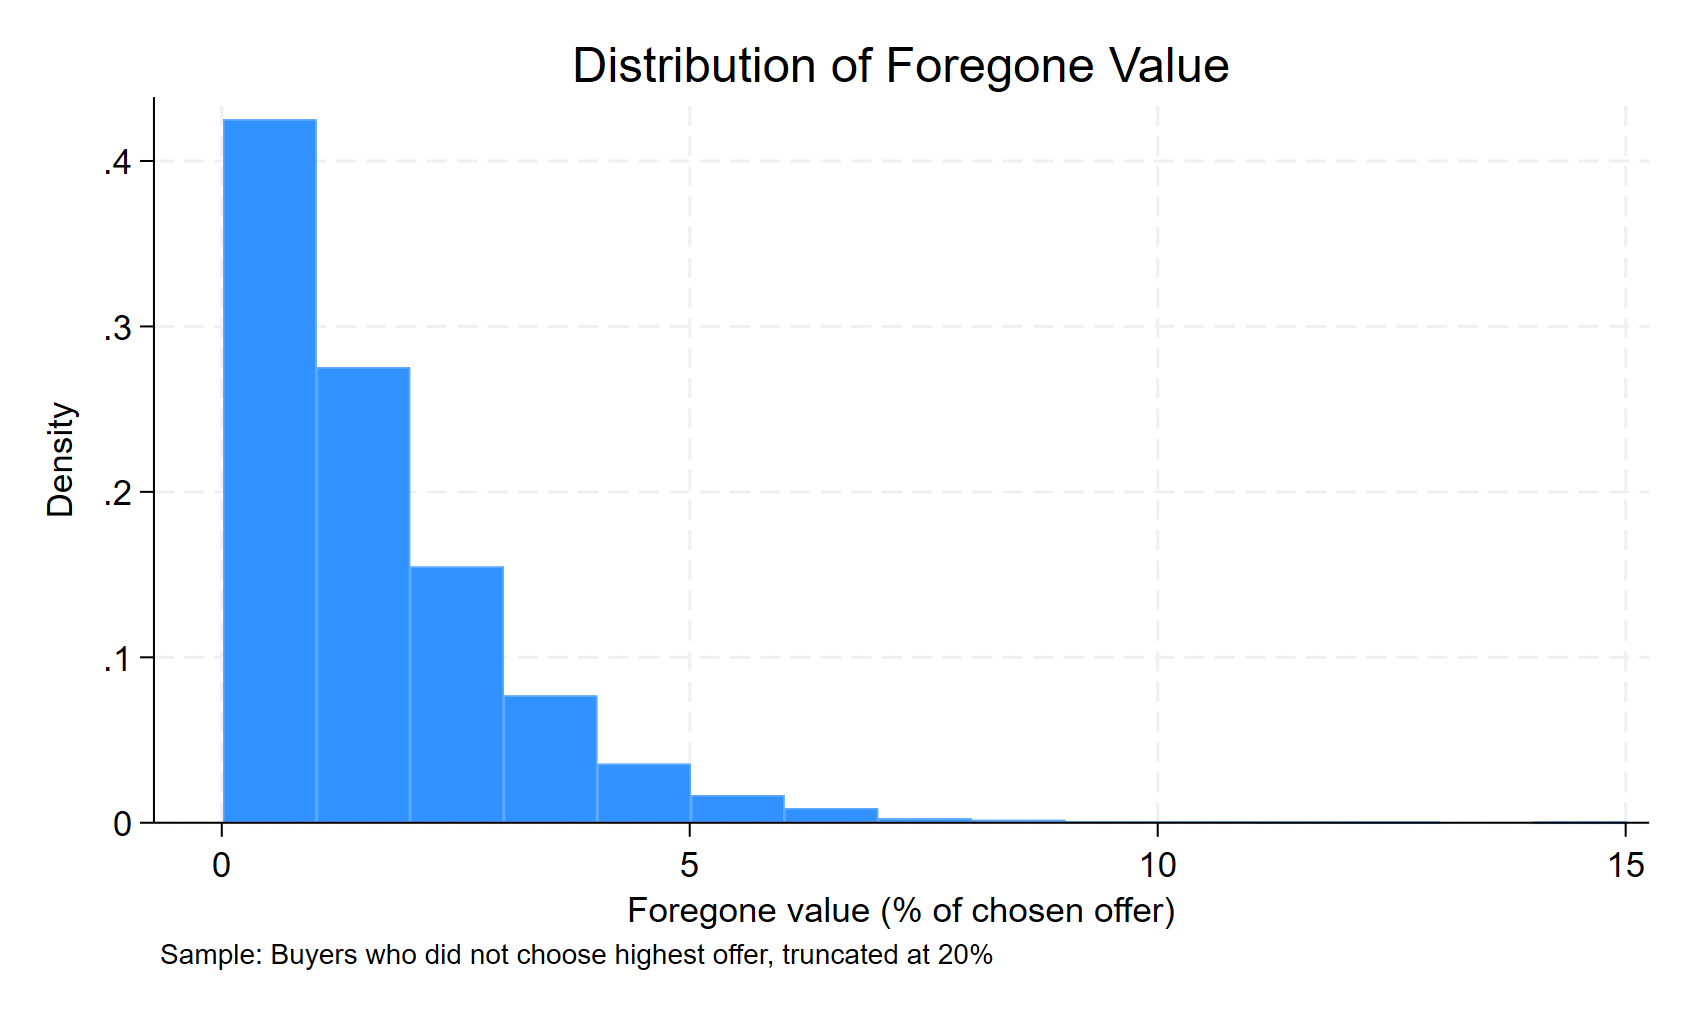
\includegraphics[scale=0.27]{figures/IE4/IE4_foregone_distribution.png} 
\end{tabular}
\end{figure} 


\begin{table}[htbp]\centering
\def\sym#1{\ifmmode^{#1}\else\(^{#1}\)\fi}
\caption{Determinants of Foregone Value}
\begin{tabular}{l*{1}{c}}
\hline\hline
            &\multicolumn{1}{c}{(1)}         \\
\hline
has\_intermediary&       0.498\sym{***}\\
            &     (0.034)         \\
[1em]
has\_external&      -0.287\sym{***}\\
            &     (0.041)         \\
[1em]
1.income\_q  &       0.000         \\
            &         (.)         \\
[1em]
2.income\_q  &      -0.680\sym{***}\\
            &     (0.048)         \\
[1em]
3.income\_q  &      -0.791\sym{***}\\
            &     (0.049)         \\
[1em]
4.income\_q  &      -0.660\sym{***}\\
            &     (0.055)         \\
[1em]
5.income\_q  &      -0.408\sym{***}\\
            &     (0.059)         \\
[1em]
n\_total\_offers&      -0.012\sym{***}\\
            &     (0.002)         \\
[1em]
\_cons      &       2.217\sym{***}\\
            &     (0.050)         \\
\hline
Obs.        &       8,342         \\
R-squared   &       0.075         \\
\hline\hline
\multicolumn{2}{l}{\footnotesize Sample: Buyers who did not choose highest offer. DV: Foregone }\\
\end{tabular}
\end{table}


%\documentclass{article}
\usepackage{multirow}
\usepackage{amsmath}
\usepackage{ulem}
\usepackage[table]{xcolor}
\begin{document}
\begin{table}[!h]
\centering
\begin{tabular}{llll}
\cline{1-4}
\multicolumn{1}{c}{} &
  \multicolumn{3}{|c}{has\_intermediary} \\
\multicolumn{1}{c}{} &
  \multicolumn{1}{|r}{0} &
  \multicolumn{1}{r}{1} &
  \multicolumn{1}{r}{Total} \\
\cline{1-4}
\multicolumn{1}{l}{5 quantiles of val\_uf\_saldo} &
  \multicolumn{1}{|r}{} &
  \multicolumn{1}{r}{} &
  \multicolumn{1}{r}{} \\
\multicolumn{1}{l}{\hspace{1em}Q1 (low)} &
  \multicolumn{1}{|r}{} &
  \multicolumn{1}{r}{} &
  \multicolumn{1}{r}{} \\
\multicolumn{1}{l}{\hspace{2em}Mean} &
  \multicolumn{1}{|r}{0.612} &
  \multicolumn{1}{r}{0.442} &
  \multicolumn{1}{r}{0.516} \\
\multicolumn{1}{l}{\hspace{2em}Number of nonmissing values} &
  \multicolumn{1}{|r}{1,612} &
  \multicolumn{1}{r}{2,088} &
  \multicolumn{1}{r}{3,700} \\
\multicolumn{1}{l}{\hspace{1em}Q2} &
  \multicolumn{1}{|r}{} &
  \multicolumn{1}{r}{} &
  \multicolumn{1}{r}{} \\
\multicolumn{1}{l}{\hspace{2em}Mean} &
  \multicolumn{1}{|r}{0.669} &
  \multicolumn{1}{r}{0.425} &
  \multicolumn{1}{r}{0.550} \\
\multicolumn{1}{l}{\hspace{2em}Number of nonmissing values} &
  \multicolumn{1}{|r}{1,868} &
  \multicolumn{1}{r}{1,791} &
  \multicolumn{1}{r}{3,659} \\
\multicolumn{1}{l}{\hspace{1em}Q3} &
  \multicolumn{1}{|r}{} &
  \multicolumn{1}{r}{} &
  \multicolumn{1}{r}{} \\
\multicolumn{1}{l}{\hspace{2em}Mean} &
  \multicolumn{1}{|r}{0.678} &
  \multicolumn{1}{r}{0.452} &
  \multicolumn{1}{r}{0.574} \\
\multicolumn{1}{l}{\hspace{2em}Number of nonmissing values} &
  \multicolumn{1}{|r}{1,963} &
  \multicolumn{1}{r}{1,681} &
  \multicolumn{1}{r}{3,644} \\
\multicolumn{1}{l}{\hspace{1em}Q4} &
  \multicolumn{1}{|r}{} &
  \multicolumn{1}{r}{} &
  \multicolumn{1}{r}{} \\
\multicolumn{1}{l}{\hspace{2em}Mean} &
  \multicolumn{1}{|r}{0.664} &
  \multicolumn{1}{r}{0.467} &
  \multicolumn{1}{r}{0.576} \\
\multicolumn{1}{l}{\hspace{2em}Number of nonmissing values} &
  \multicolumn{1}{|r}{2,028} &
  \multicolumn{1}{r}{1,612} &
  \multicolumn{1}{r}{3,640} \\
\multicolumn{1}{l}{\hspace{1em}Q5 (high)} &
  \multicolumn{1}{|r}{} &
  \multicolumn{1}{r}{} &
  \multicolumn{1}{r}{} \\
\multicolumn{1}{l}{\hspace{2em}Mean} &
  \multicolumn{1}{|r}{0.526} &
  \multicolumn{1}{r}{0.478} &
  \multicolumn{1}{r}{0.505} \\
\multicolumn{1}{l}{\hspace{2em}Number of nonmissing values} &
  \multicolumn{1}{|r}{2,036} &
  \multicolumn{1}{r}{1,613} &
  \multicolumn{1}{r}{3,649} \\
\multicolumn{1}{l}{\hspace{1em}Total} &
  \multicolumn{1}{|r}{} &
  \multicolumn{1}{r}{} &
  \multicolumn{1}{r}{} \\
\multicolumn{1}{l}{\hspace{2em}Mean} &
  \multicolumn{1}{|r}{0.629} &
  \multicolumn{1}{r}{0.452} &
  \multicolumn{1}{r}{0.544} \\
\multicolumn{1}{l}{\hspace{2em}Number of nonmissing values} &
  \multicolumn{1}{|r}{9,507} &
  \multicolumn{1}{r}{8,785} &
  \multicolumn{1}{r}{18,292} \\
\cline{1-4}
\end{tabular}
\end{table}
\end{document}

%\input{Tables/IE4/IE4_.tex}


\newpage

\subsection{TBD}
\begin{table}[htbp]\centering
\def\sym#1{\ifmmode^{#1}\else\(^{#1}\)\fi}
\caption{Rank of Accepted External Offers (1=Highest)}
\begin{tabular}{l*{1}{cccccc}}
\hline\hline
            &        mean&         p50&          sd&         min&         max&       count\\
\hline
offer\_rank  &        2.90&            &        3.18&           1&          39&       13683\\
offer\_rank\_pct&       14.77&            &       21.98&           0&          97&       13666\\
\hline
\(N\)       &       13683&            &            &            &            &            \\
\hline\hline
\end{tabular}
\end{table}


  \begin{figure}[H]
\caption{}
 \label{fig:ie4_11}
\centering{}%
\begin{tabular}{cc}
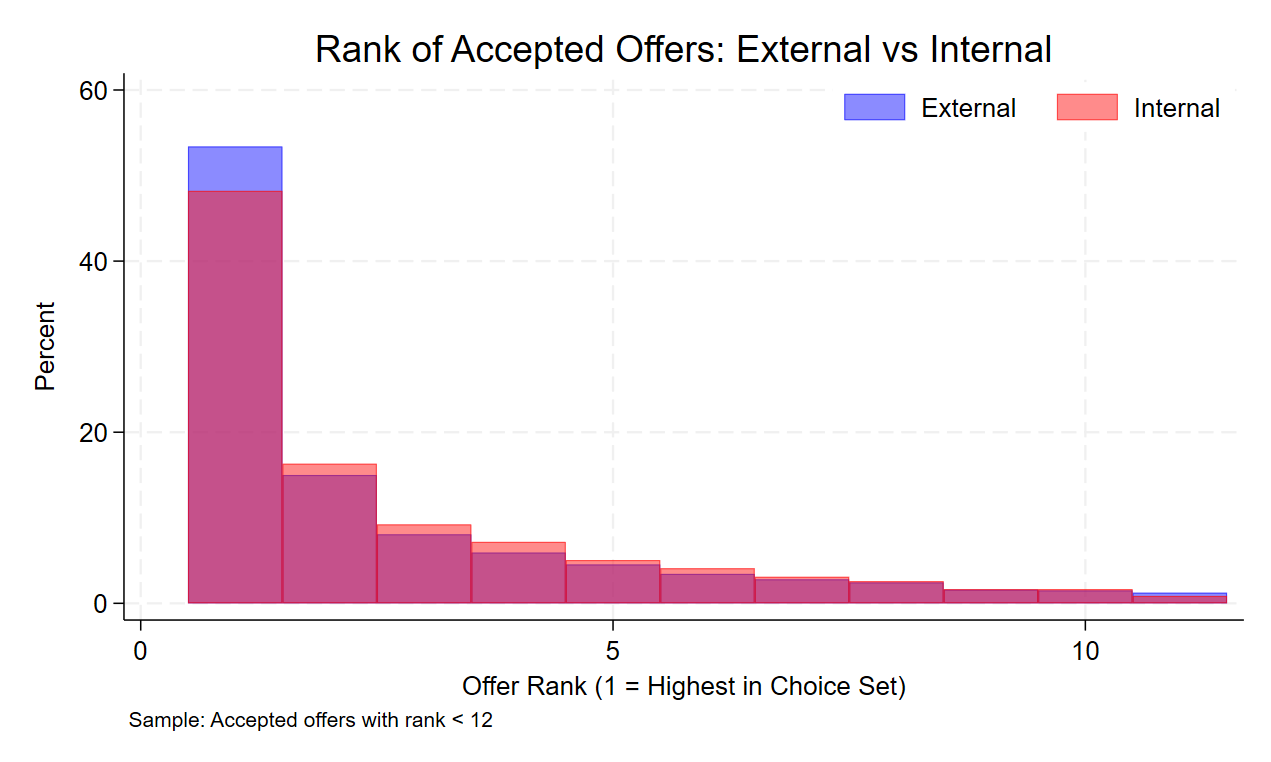
\includegraphics[scale=0.27]{figures/IE4/IE4_rank_of_accepted_external.png} 
\end{tabular}
\end{figure} 

\begin{table}[htbp]\centering
\def\sym#1{\ifmmode^{#1}\else\(^{#1}\)\fi}
\caption{Rank Comparison: External vs Internal Accepted Offers}
\begin{tabular}{l*{1}{cccc}}
\hline\hline
            &        mean&         p50&          sd&       count\\
\hline
External    &            &            &            &            \\
offer\_rank  &        2.90&         1.0&        3.18&       13683\\
offer\_rank\_pct&       14.74&         0.0&       21.98&       13666\\
\hline
Internal    &            &            &            &            \\
offer\_rank  &        2.98&         2.0&        3.11&        4609\\
offer\_rank\_pct&       19.82&         8.3&       26.81&        4438\\
\hline
Total       &            &            &            &            \\
offer\_rank  &        2.92&         1.0&        3.17&       18292\\
offer\_rank\_pct&       15.98&         0.0&       23.36&       18104\\
\hline
\(N\)       &       18292&            &            &            \\
\hline\hline
\end{tabular}
\end{table}



\begin{table}[htbp]\centering
\def\sym#1{\ifmmode^{#1}\else\(^{#1}\)\fi}
\caption{Share of Accepted Offers in Top Rankings}
\begin{tabular}{l*{6}{c}}
\hline\hline
            &        mean&        mean&        mean&        mean&        mean&        mean\\
\hline
\hline
\(N\)       &       18292&       18292&       18292&       18292&       18292&        8342\\
\hline\hline
\end{tabular}
\end{table}





  \begin{figure}[H]
\caption{}
 \label{fig:ie4_11}
\centering{}%
\begin{tabular}{cc}
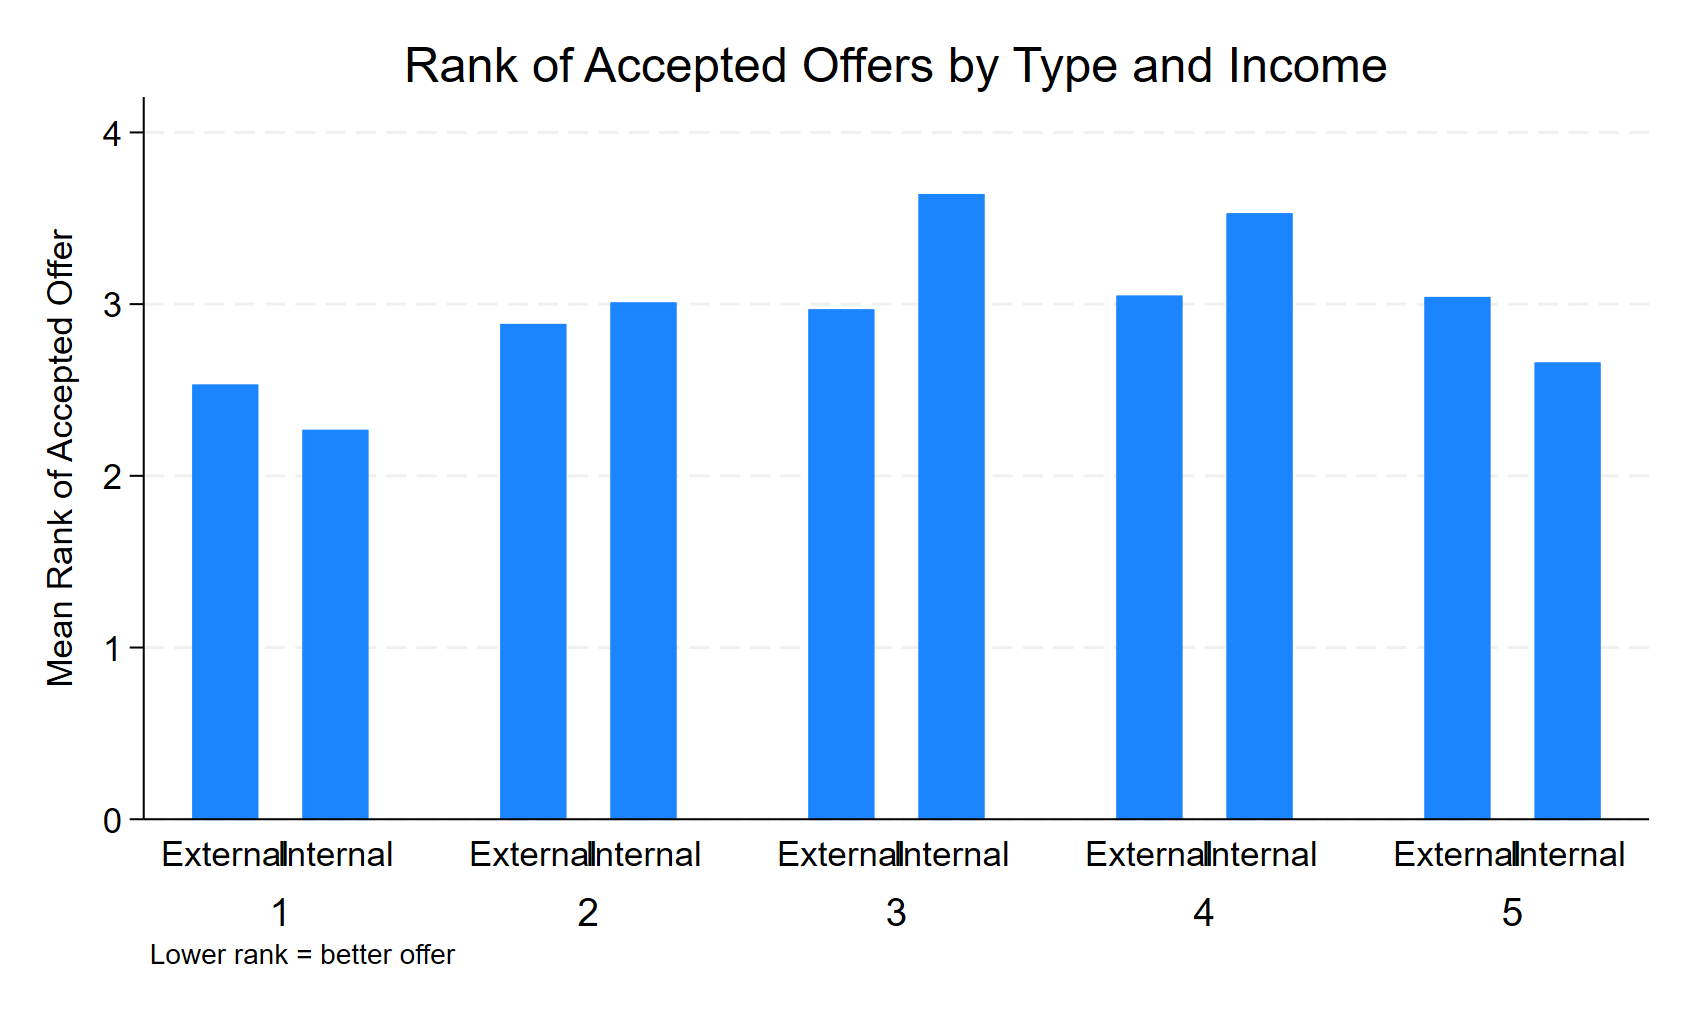
\includegraphics[scale=0.17]{figures/IE4/IE4_rank_by_type_income.png} 
\end{tabular}
\end{figure} 


\newpage


  \begin{figure}[H]
\caption{}
 \label{fig:ie4_11}
\centering{}%
\begin{tabular}{cc}
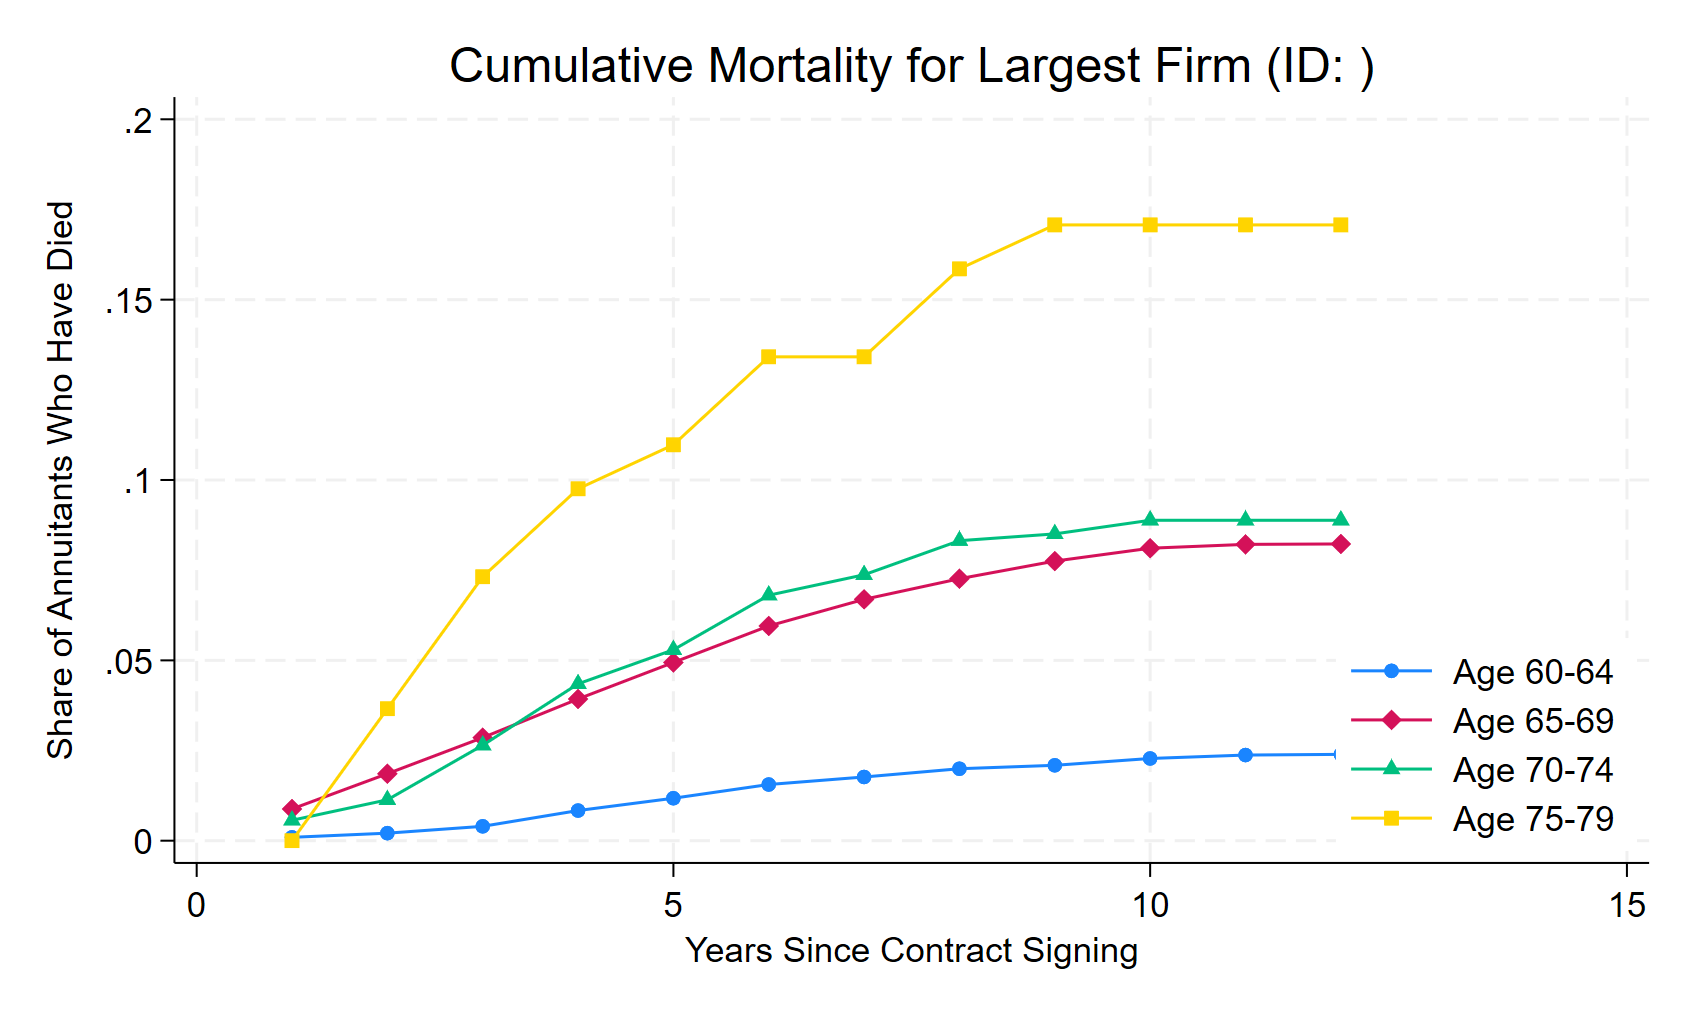
\includegraphics[scale=0.27]{figures/IE4/IE4_mortality_curves_by_age.png} 
\end{tabular}
\end{figure} 


   \begin{figure}[H]
\caption{}
 \label{fig:ie4_11}
\centering{}%
\begin{tabular}{cc}
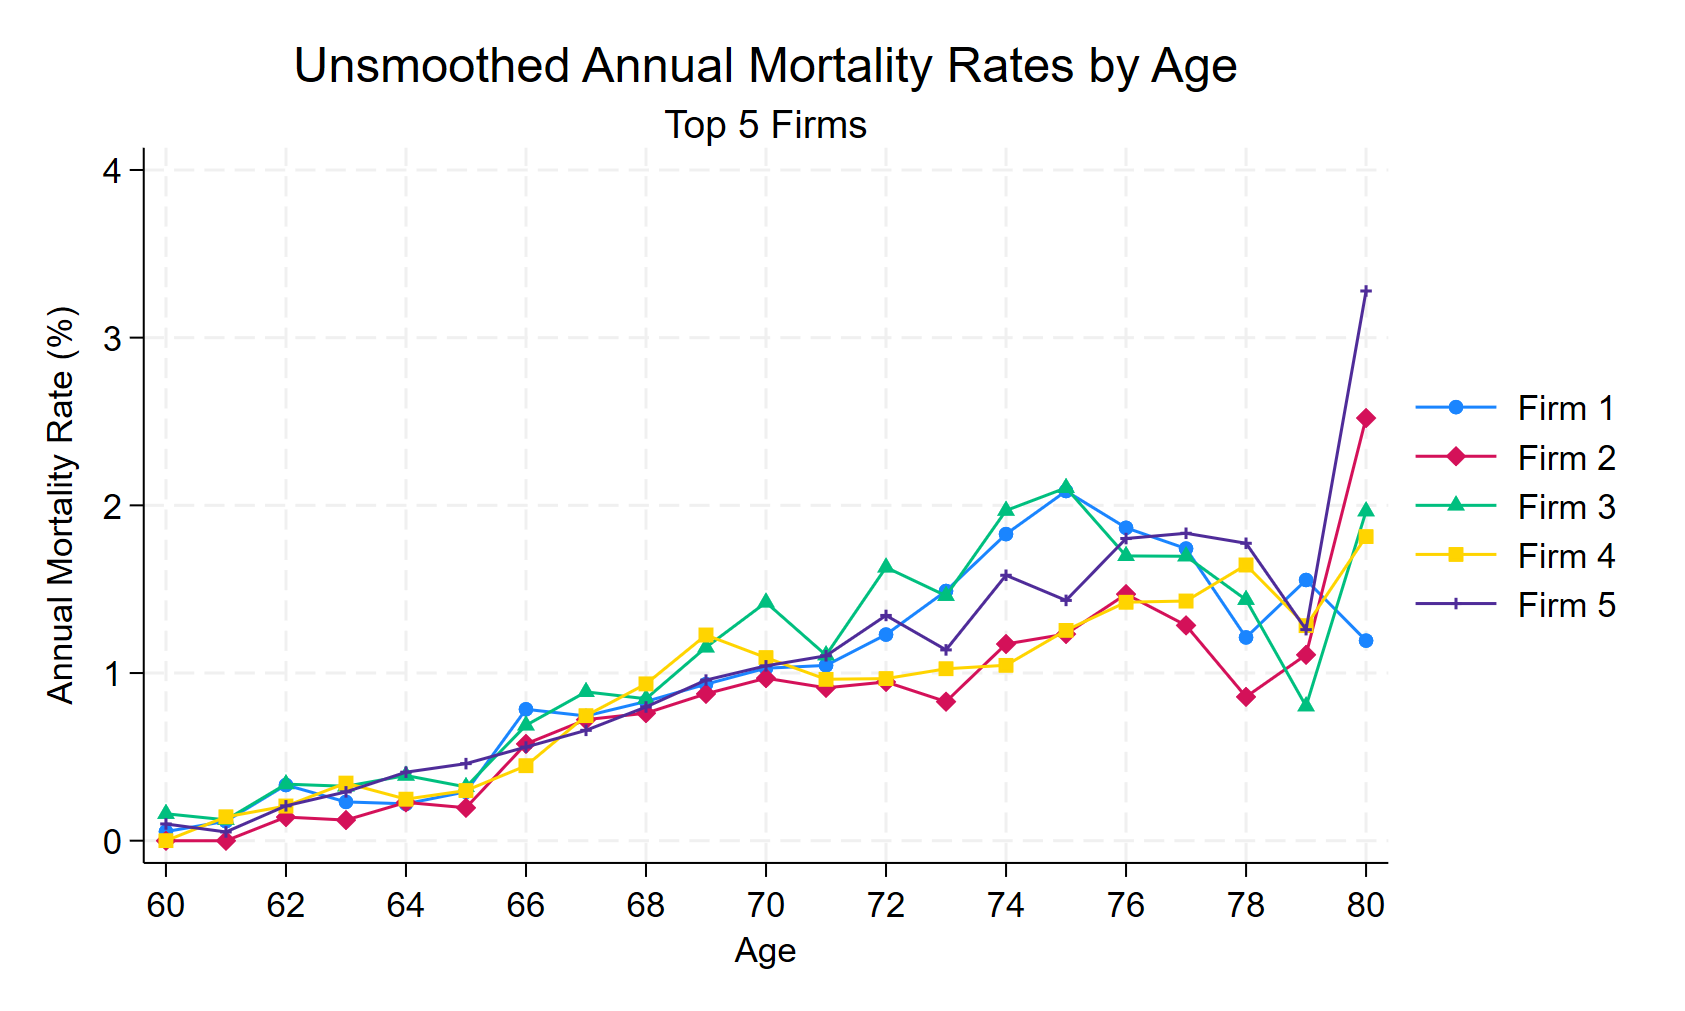
\includegraphics[scale=0.17]{figures/IE4/IE4_mortality_rates_unsmoothed.png} 
& 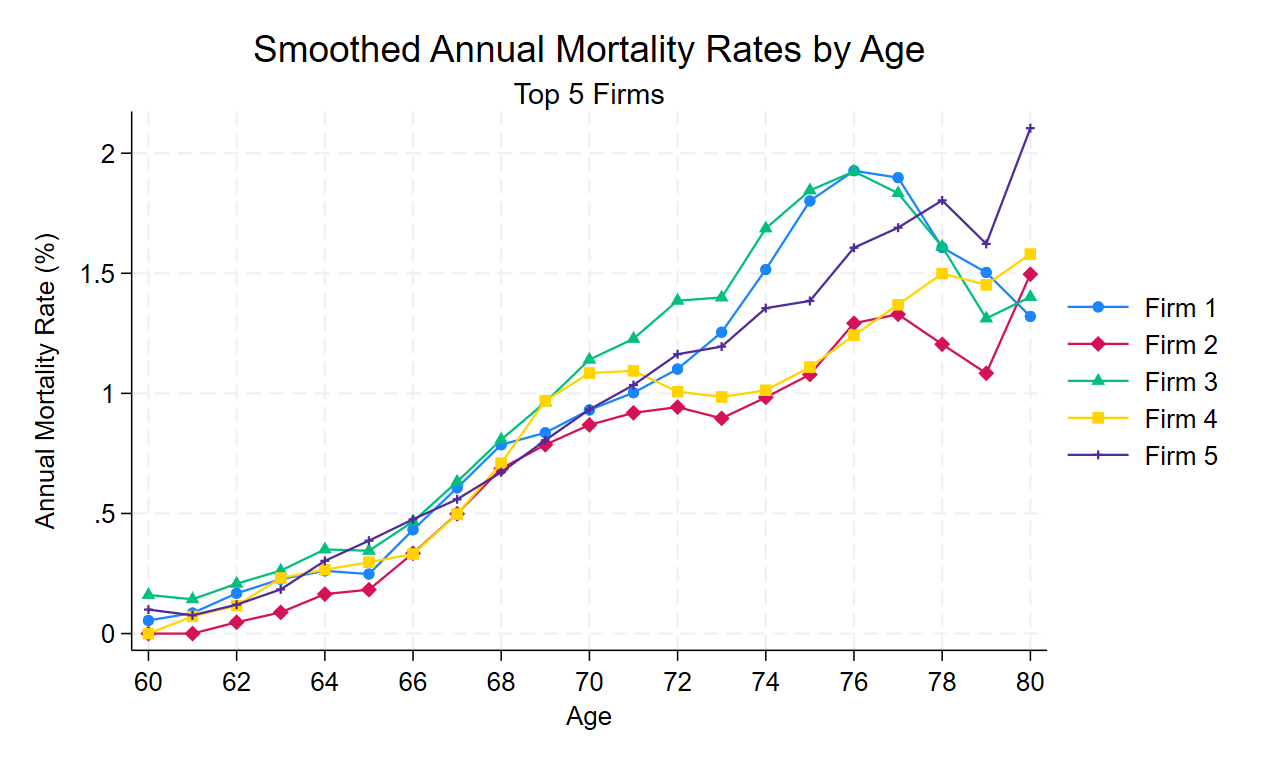
\includegraphics[scale=0.17]{figures/IE4/IE4_mortality_rates_smoothed.png} 
\end{tabular}
\end{figure} 
 


 
  \begin{figure}[H]
\caption{}
 \label{fig:ie4_11}
\centering{}%
\begin{tabular}{cc}
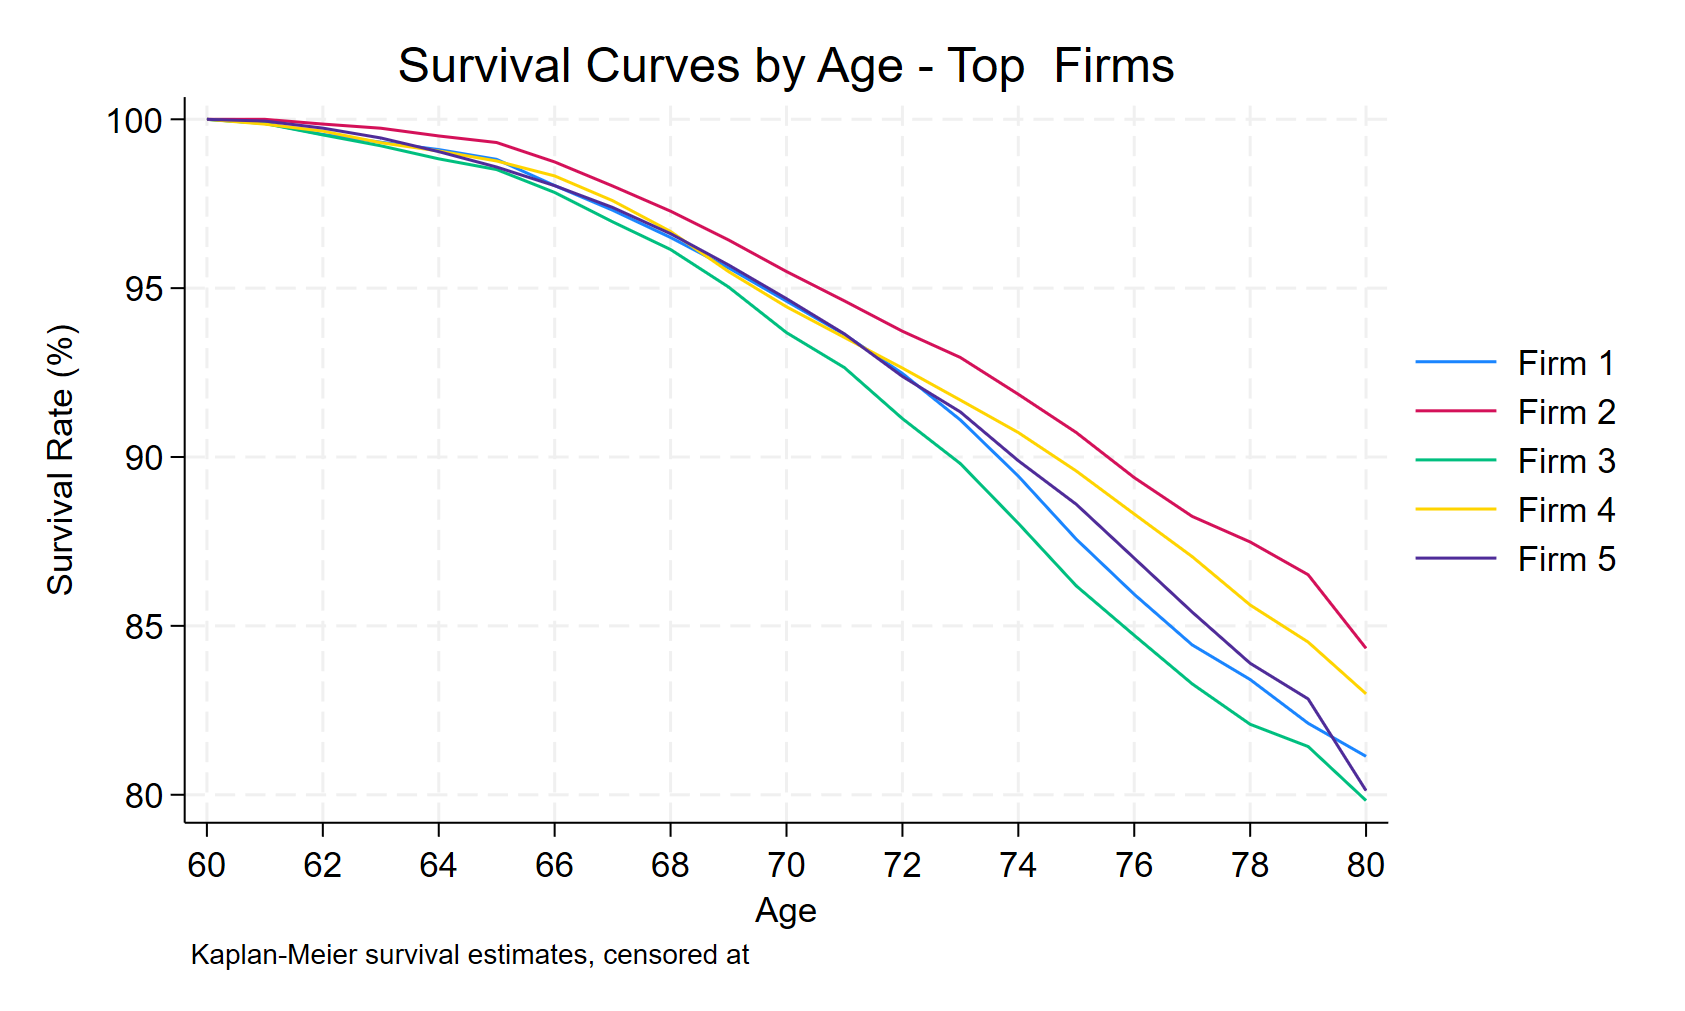
\includegraphics[scale=0.2]{figures/IE4/IE4_survival_curves_by_age_top_firms.png} 
\end{tabular}
\end{figure} 


\end{document}